\documentclass[10pt]{article}

% Essential packages
\usepackage[utf8]{inputenc}
\usepackage[T1]{fontenc}
\usepackage[french]{babel}
\usepackage{microtype} % Improved typography for better text rendering
\usepackage{lmodern} % Latin Modern fonts for better rendering
\usepackage{fontawesome5} % Modern icons
\usepackage{ragged2e} % Better text alignment

% Layout and design packages
\usepackage{geometry}
\usepackage{fancyhdr}
\usepackage{titlesec}
\usepackage{titletoc} % Table of contents customization
\usepackage{tcolorbox}
\usepackage{mdframed}
\usepackage{changepage} % For adjustwidth environment
\usepackage{pdflscape} % For landscape pages
\usepackage{float}
\usepackage{wrapfig} % Wrap text around figures

% Math and graphics packages
\usepackage{graphicx}
\usepackage{amsmath}
\usepackage{amsfonts}
\usepackage{amssymb}
\usepackage{tikz} % For diagrams and graphics
\usetikzlibrary{positioning, arrows, shapes, backgrounds, fit}

% Utilities packages
\usepackage{enumitem}
\usepackage{caption}
\usepackage{subcaption} % For subfigures
\usepackage{booktabs}
\usepackage{array}
\usepackage{tabularx}
\usepackage{multirow}
\usepackage{colortbl}
\usepackage{xcolor}

% Modern link styling with hyperref (should be loaded last)
\usepackage{hyperref}

% Page geometry with more modern margins
\geometry{a4paper, margin=1in, headheight=25pt, footskip=15pt}

% Modern color palette
\definecolor{primary}{RGB}{30, 136, 229}       % Blue (primary brand color)
\definecolor{secondary}{RGB}{36, 178, 146}     % Teal (secondary accent)
\definecolor{tertiary}{RGB}{175, 122, 197}     % Purple (tertiary accent)
\definecolor{background}{RGB}{250, 250, 252}   % Light background
\definecolor{surface}{RGB}{255, 255, 255}      % Surface color
\definecolor{darktext}{RGB}{33, 37, 41}        % Primary text
\definecolor{lighttext}{RGB}{108, 117, 125}    % Secondary text
\definecolor{danger}{RGB}{220, 53, 69}         % Error/danger color
\definecolor{success}{RGB}{40, 167, 69}        % Success color
\definecolor{warning}{RGB}{255, 193, 7}        % Warning color
\definecolor{info}{RGB}{23, 162, 184}          % Info color
\definecolor{lightgray}{RGB}{248, 249, 250}    % Light gray for backgrounds
\definecolor{bordercolor}{RGB}{233, 236, 239}  % Border color

% Modern header and footer styling
\pagestyle{fancy}
\fancyhf{}
\fancyhead[L]{\raisebox{-1.5pt}{\colorbox{primary}{\textcolor{white}{\bfseries\sffamily\small DIGITAL BANKING}}}}
\fancyhead[R]{\textcolor{lighttext}{\sffamily\small\leftmark}}
\fancyfoot[C]{\textcolor{primary}{\rule{1cm}{1pt}}\quad\textcolor{darktext}{\thepage}\quad\textcolor{primary}{\rule{1cm}{1pt}}}
\renewcommand{\headrulewidth}{0pt}
\renewcommand{\footrulewidth}{0pt}
\fancypagestyle{plain}{%
  \fancyhf{}%
  \fancyfoot[C]{\textcolor{primary}{\rule{1cm}{1pt}}\quad\textcolor{darktext}{\thepage}\quad\textcolor{primary}{\rule{1cm}{1pt}}}%
  \renewcommand{\headrulewidth}{0pt}%
  \renewcommand{\footrulewidth}{0pt}%
}

% Section styling with titlesec
\titleformat{\section}
{\Large\bfseries\sffamily\color{primary}}
{}
{0em}
{\filcenter\MakeUppercase}
% [\titlerule[1pt]]

\titleformat{\subsection}
{\large\bfseries\sffamily\color{secondary}}
{\thesubsection}
{0.75em}
{}
[\vspace{-0.5em}\rule{\textwidth}{0.5pt}]

\titleformat{\subsubsection}
{\normalsize\bfseries\sffamily\color{tertiary}}
{\thesubsubsection}
{0.5em}
{}

% Table of contents formatting
\renewcommand{\contentsname}{\centerline{\sffamily\Large\bfseries\color{primary}TABLE DES MATIÈRES}}

\titlecontents{section}
[0em]
{\vspace{0.5em}\bfseries\sffamily\color{primary}}
{\contentslabel{2em}}
{}
{\hfill\contentspage}
[\vspace{0.25em}]

\titlecontents{subsection}
[2em]
{\sffamily\color{secondary}}
{\contentslabel{2.5em}}
{}
{\titlerule*[0.5em]{.}\contentspage}
[\vspace{0.25em}]

\titlecontents{subsubsection}
[4.5em]
{\sffamily\color{lighttext}\small}
{\contentslabel{3em}}
{}
{\titlerule*[0.5em]{.}\contentspage}

% Caption styling
\captionsetup{
    format=hang,
    font={normalsize,sf},
    labelfont={bf,color=primary},
    textfont={color=darktext},
    margin=15pt,
    labelsep=quad,
    justification=centering,
    skip=10pt
}

% Hyperlink styling
\hypersetup{
    colorlinks=true,
    linkcolor=primary,
    filecolor=secondary,
    urlcolor=info,
    citecolor=tertiary,
    pdfborder={0 0 0},
    breaklinks=true,
    pdfauthor={Youssef Faik},
    pdftitle={Rapport Technique - Digital Banking},
    pdfsubject={Documentation Technique pour Application Bancaire},
    pdfkeywords={Digital Banking, Spring Boot, Angular, API, Documentation}
}

% Define custom tcolorbox styles
\tcbuselibrary{skins, breakable, theorems}

% Primary box style
\newtcolorbox{primarybox}[1][]{
    enhanced,
    breakable,
    colback=lightgray,
    colframe=primary,
    arc=5pt,
    boxrule=1pt,
    fonttitle=\bfseries\sffamily\color{white},
    coltitle=white,
    colbacktitle=primary,
    attach boxed title to top left={xshift=0.5cm, yshift=-\tcboxedtitleheight/2},
    boxed title style={arc=3pt, boxrule=0pt},
    #1
}

% Secondary box style
\newtcolorbox{secondarybox}[1][]{
    enhanced,
    breakable,
    colback=white,
    colframe=secondary,
    arc=5pt,
    boxrule=1pt,
    fonttitle=\bfseries\sffamily\color{white},
    coltitle=white,
    colbacktitle=secondary,
    attach boxed title to top left={xshift=0.5cm, yshift=-\tcboxedtitleheight/2},
    boxed title style={arc=3pt, boxrule=0pt},
    #1
}

% Info box style
\newtcolorbox{infobox}[1][]{
    enhanced,
    breakable,
    colback=white,
    colframe=info,
    arc=5pt,
    boxrule=1pt,
    fonttitle=\bfseries\sffamily\color{white},
    coltitle=white,
    colbacktitle=info,
    attach boxed title to top left={xshift=0.5cm, yshift=-\tcboxedtitleheight/2},
    boxed title style={arc=3pt, boxrule=0pt},
    #1
}

% Warning box style
\newtcolorbox{warningbox}[1][]{
    enhanced,
    breakable,
    colback=white,
    colframe=warning,
    arc=5pt,
    boxrule=1pt,
    fonttitle=\bfseries\sffamily\color{white},
    coltitle=white,
    colbacktitle=warning,
    attach boxed title to top left={xshift=0.5cm, yshift=-\tcboxedtitleheight/2},
    boxed title style={arc=3pt, boxrule=0pt},
    #1
}

% Success box style
\newtcolorbox{successbox}[1][]{
    enhanced,
    breakable,
    colback=white,
    colframe=success,
    arc=5pt,
    boxrule=1pt,
    fonttitle=\bfseries\sffamily\color{white},
    coltitle=white,
    colbacktitle=success,
    attach boxed title to top left={xshift=0.5cm, yshift=-\tcboxedtitleheight/2},
    boxed title style={arc=3pt, boxrule=0pt},
    #1
}

% Image frame style
\newtcolorbox{imagebox}[1][]{
    enhanced,
    colback=white,
    colframe=bordercolor,
    arc=8pt,
    boxrule=1.5pt,
    sharp corners=false,
    left=12pt,
    right=12pt,
    top=12pt,
    bottom=12pt,
    drop shadow={shadow xshift=2pt, shadow yshift=-2pt, opacity=0.15},
    #1
}

\title{\Huge\textbf{\textcolor{primary}{Rapport de l'Application Digital Banking}}}
\author{\large\textcolor{darktext}{Youssef Faik}}
\date{\large\textcolor{darktext}{Mai 2025}}

% Input custom commands
% Custom commands for consistent formatting
\newcommand{\sectiondivider}{
    \begin{center}
        \textcolor{primary}{\rule{0.3\textwidth}{1pt}}
        \quad\faChevronDown\quad
        \textcolor{primary}{\rule{0.3\textwidth}{1pt}}
    \end{center}
}

\newcommand{\featureheading}[1]{
    \vspace{0.5em}
    \noindent\textcolor{primary}{\textbf{\sffamily\large #1}}
    \vspace{0.5em}
}

\newcommand{\technote}[1]{
    \begin{secondarybox}[title=Note technique]
        \sffamily\small #1
    \end{secondarybox}
}

\newcommand{\keypoint}[1]{
    \begin{primarybox}[title=Point clé]
        \sffamily #1
    \end{primarybox}
}

% Command for code snippets
\newcommand{\codesnippet}[2]{
    \begin{tcolorbox}[
        colback=darktext!5!white,
        colframe=darktext!50!white,
        arc=3pt,
        title=\textcolor{darktext}{\textbf{\sffamily #1}},
        fonttitle=\small\sffamily,
        boxrule=0.5pt,
        left=5pt,right=5pt,top=5pt,bottom=5pt
    ]
    \small\ttfamily #2
    \end{tcolorbox}
}

% Command for API endpoint documentation
\newcommand{\apiendpoint}[4]{
    \begin{tcolorbox}[
        enhanced,
        colback=lightgray,
        colframe=tertiary,
        arc=3pt,
        title=\textcolor{white}{\textbf{\sffamily #1 #2}},
        fonttitle=\sffamily,
        coltitle=white,
        colbacktitle=tertiary,
        boxrule=0.5pt,
        left=5pt,right=5pt,top=5pt,bottom=5pt
    ]
    \small\sffamily
    \textbf{Description:} #3 \\
    \textbf{Réponse:} \texttt{#4}
    \end{tcolorbox}
}

% Command for feature showcase
\newcommand{\featureshowcase}[3]{
    \begin{minipage}{\textwidth}
        \begin{minipage}{0.65\textwidth}
            \begin{secondarybox}[title=#1]
                \sffamily #2
            \end{secondarybox}
        \end{minipage}
        \hfill
        \begin{minipage}{0.3\textwidth}
            \begin{imagebox}
                \includegraphics[width=\textwidth]{#3}
            \end{imagebox}
        \end{minipage}
    \end{minipage}
}

% Command for technology badge
\newcommand{\techbadge}[2]{
    \tikz[baseline=(char.base)]{
        \node[
            fill=#2!10,
            draw=#2,
            rounded corners=3pt,
            inner sep=2pt,
            text=#2
        ] (char) {#1};
    }
}

% Command for step-by-step process
\newcommand{\processstep}[2]{
    \begin{tcolorbox}[
        enhanced,
        colback=white,
        colframe=secondary,
        leftrule=3pt,
        rightrule=0pt,
        toprule=0pt,
        bottomrule=0pt,
        arc=0pt,
        left=8pt
    ]
        \textbf{\sffamily\textcolor{secondary}{Étape #1:}} \sffamily #2
    \end{tcolorbox}
}

% Command for comparison table header row
\newcommand{\comparisonheader}[3]{
    \rowcolor{primary!20}
    \textbf{\sffamily #1} & \textbf{\sffamily #2} & \textbf{\sffamily #3} \\
}

% Command for bullet with icon
\newcommand{\iconbullet}[2]{
    \noindent\textcolor{primary}{#1} \sffamily #2 \\
}

% Command for feature card
\newcommand{\featurecard}[4]{
    \begin{tcolorbox}[
        enhanced,
        colback=#3!5,
        colframe=#3,
        arc=5pt,
        title=\textcolor{white}{#1 \textbf{\sffamily #2}},
        fonttitle=\sffamily,
        coltitle=white,
        colbacktitle=#3,
        boxrule=0.5pt,
        left=8pt,right=8pt,top=8pt,bottom=8pt
    ]
        \sffamily\small #4
    \end{tcolorbox}
}
}

% Command for timeline entry
\newcommand{\timelineentry}[3]{
    \begin{minipage}{\textwidth}
        \begin{tikzpicture}
            \filldraw[fill=#3!20, draw=#3] (0,0) circle (0.4cm);
            \node at (0,0) {\textcolor{#3}{\Large\bfseries #1}};
            \draw[thick, #3] (0.4,0) -- (0.7,0);
            \node[anchor=west, text width=\textwidth-1cm] at (0.8,0) {\textbf{\sffamily\textcolor{#3}{#2}}};
        \end{tikzpicture}
    \end{minipage}
    \vspace{0.2cm}
}

% Command for technology stack item
\newcommand{\techstack}[3]{
    \begin{tikzpicture}
        \node[
            draw=#2,
            fill=#2!5,
            rounded corners=5pt,
            minimum width=3cm,
            minimum height=1.5cm
        ] {
            \begin{tabular}{c}
                \textcolor{#2}{#1} \\
                \textbf{\sffamily\small #3}
            \end{tabular}
        };
    \end{tikzpicture}
}


\begin{document}

% Modern title page
\begin{titlepage}
    \thispagestyle{empty}
    
    % Header
    \begin{center}
        \vspace*{-1cm}
        
        \vspace{1cm}
        {\fontsize{30}{36}\selectfont\sffamily\bfseries\textcolor{primary}{DIGITAL BANKING}\par}
        \vspace{0.3cm}
        {\large\sffamily\textcolor{lighttext}{DOCUMENTATION TECHNIQUE}\par}
        
        \vspace{2cm}
    \end{center}
    
    % Main content box
    \begin{center}
        \begin{tcolorbox}[
            enhanced,
            width=0.85\textwidth,
            colback=background,
            colframe=primary,
            arc=10pt,
            boxrule=1pt,
            boxsep=15pt,
            left=20pt,
            right=20pt
        ]
            \begin{center}
                \vspace{0.5cm}
                {\LARGE\sffamily\bfseries\textcolor{primary}{RAPPORT COMPLET}\par}
                \vspace{0.3cm}
                {\large\sffamily\textcolor{darktext}{Architecture, Fonctionnalités \& API}\par}
                \vspace{1cm}
            \end{center}
        \end{tcolorbox}
    \end{center}
    
    \vfill
    
    % Footer
    \begin{center}
        \begin{tcolorbox}[
            enhanced,
            width=0.9\textwidth,
            colback=white,
            colframe=bordercolor,
            arc=5pt,
            boxrule=0.5pt,
            boxsep=10pt
        ]
            \begin{center}
                {\large\sffamily\bfseries\textcolor{primary}{Youssef Faik}\par}
                \vspace{0.2cm}
                {\small\sffamily\textcolor{lighttext}{June 2025}\par}
                \vspace{0.3cm}
                
                \begin{tabular}{cccc}
                    \textcolor{primary}{\faCode} & 
                    \textcolor{secondary}{\faServer} & 
                    \textcolor{tertiary}{\faDatabase} & 
                    \textcolor{info}{\faShieldAlt} \\
                    Angular & Spring Boot & MySQL & JWT Auth \\
                \end{tabular}
            \end{center}
        \end{tcolorbox}
    \end{center}
    
    \vspace{1cm}
\end{titlepage}

% Réinitialiser le style de page après la page de titre
\pagestyle{fancy}

% Abstract with modern styling
\begin{abstract}
\begin{primarybox}[title=Résumé]
\sffamily\justify
Ce rapport détaille les fonctionnalités clés de l'application \textbf{Digital Banking}, une plateforme bancaire moderne conçue pour offrir une expérience numérique intuitive et efficace. 

Le document commence par une présentation détaillée de l'architecture en couches de l'application, suivie d'une exploration approfondie des processus d'authentification sécurisée, de la gestion complète des clients et des comptes bancaires, ainsi que de l'ensemble des opérations bancaires courantes (débit, crédit, virement).

Une section est également consacrée à la documentation API interactive générée avec Swagger/OpenAPI, permettant aux développeurs de comprendre et de tester facilement l'ensemble des services backend.

Chaque fonctionnalité est illustrée par des captures d'écran détaillées pour une compréhension visuelle immédiate des interfaces et des flux utilisateur.
\end{primarybox}
\end{abstract}

% Table of contents with modern styling
\begingroup
\hypersetup{linkcolor=darktext}
\tableofcontents
\endgroup

\newpage

\section{Introduction}
\sectiondivider

\begin{secondarybox}[title=Présentation générale]
\sffamily\justify
L'application \textbf{Digital Banking} représente une solution technologique avancée visant à moderniser et simplifier l'interaction des utilisateurs avec les services bancaires traditionnels.

Cette plateforme numérique offre une interface utilisateur intuitive et responsive, développée avec les technologies web les plus récentes, permettant aux utilisateurs d'effectuer l'ensemble de leurs opérations bancaires de manière sécurisée et efficace.

Le présent document a pour objectif de fournir une documentation technique complète de l'application, expliquant son architecture, ses fonctionnalités principales et la manière dont ses API sont exposées et documentées.
\end{secondarybox}

\subsection{Objectifs de l'Application}

\featureheading{Une Plateforme Bancaire Intégrée et Moderne}

\begin{itemize}[leftmargin=20pt, itemsep=5pt]
    \item \textbf{\textcolor{primary}{Modernisation}} : Proposer une interface utilisateur contemporaine, intuitive et ergonomique suivant les meilleures pratiques UX/UI
    
    \item \textbf{\textcolor{primary}{Sécurité}} : Garantir la protection des données et des transactions via des mécanismes d'authentification et d'autorisation robustes basés sur JWT
    
    \item \textbf{\textcolor{primary}{Simplicité}} : Offrir une expérience utilisateur fluide et intuitive, minimisant la courbe d'apprentissage
    
    \item \textbf{\textcolor{primary}{Complétude}} : Couvrir l'ensemble des besoins bancaires quotidiens des utilisateurs dans une interface unifiée
    
    \item \textbf{\textcolor{primary}{Transparence API}} : Fournir une documentation API claire et interactive via Swagger pour faciliter l'intégration et l'évolution
    
    \item \textbf{\textcolor{primary}{Modularité}} : Adopter une architecture en couches clairement définie pour favoriser la maintenabilité et l'extensibilité du code
\end{itemize}

\technote{
L'application a été conçue selon les principes de l'architecture orientée services (SOA), avec une séparation nette entre le frontend Angular et le backend Spring Boot. Cette approche permet d'isoler les préoccupations et d'optimiser indépendamment les différentes parties du système.
}

\subsection{Technologies et Stack Technique}

\begin{tcolorbox}[
    enhanced,
    colback=white,
    colframe=bordercolor,
    arc=0pt,
    boxrule=0.5pt,
    boxsep=10pt,
    title=\textcolor{primary}{\textbf{\sffamily Stack Technique}},
    fonttitle=\large\sffamily
]
\begin{tabularx}{\textwidth}{>{\raggedright\arraybackslash}X>{\raggedright\arraybackslash}X}
\textbf{\textcolor{primary}{Frontend}} & \textbf{\textcolor{secondary}{Backend}} \\
\hline
\begin{itemize}[leftmargin=15pt, itemsep=3pt]
    \item Angular 17
    \item TypeScript 5
    \item HTML5/SCSS
    \item Bootstrap 5
    \item Chart.js
    \item RxJS
\end{itemize} &
\begin{itemize}[leftmargin=15pt, itemsep=3pt]
    \item Spring Boot 3.4
    \item Spring Security
    \item Spring Data JPA
    \item Java 21
    \item MySQL 8
    \item Swagger/OpenAPI 3
\end{itemize} \\
\end{tabularx}
\end{tcolorbox}

\newpage

% --- SECTION FOR ARCHITECTURE DIAGRAM ---
\section{Architecture Générale de l'Application}
\label{sec:architecture}

\sectiondivider

\begin{primarybox}[title=Vue d'ensemble]
    L'application Digital Banking est conçue selon une architecture client-serveur moderne, 
    tirant parti des frameworks \techbadge{Angular}{primary} pour le frontend et 
    \techbadge{Spring Boot}{secondary} pour le backend. Cette séparation claire des préoccupations 
    permet une meilleure maintenabilité, évolutivité et des cycles de développement indépendants 
    pour l'interface utilisateur et la logique métier.
    
    Le diagramme présenté en Figure \ref{fig:architecture_diagram} illustre les principaux 
    composants et leurs interactions.
\end{primarybox}

\begin{landscape}
\begin{figure}[p] % Using [p] for page of floats, suitable for landscape
    \centering
    \begin{imagebox}
        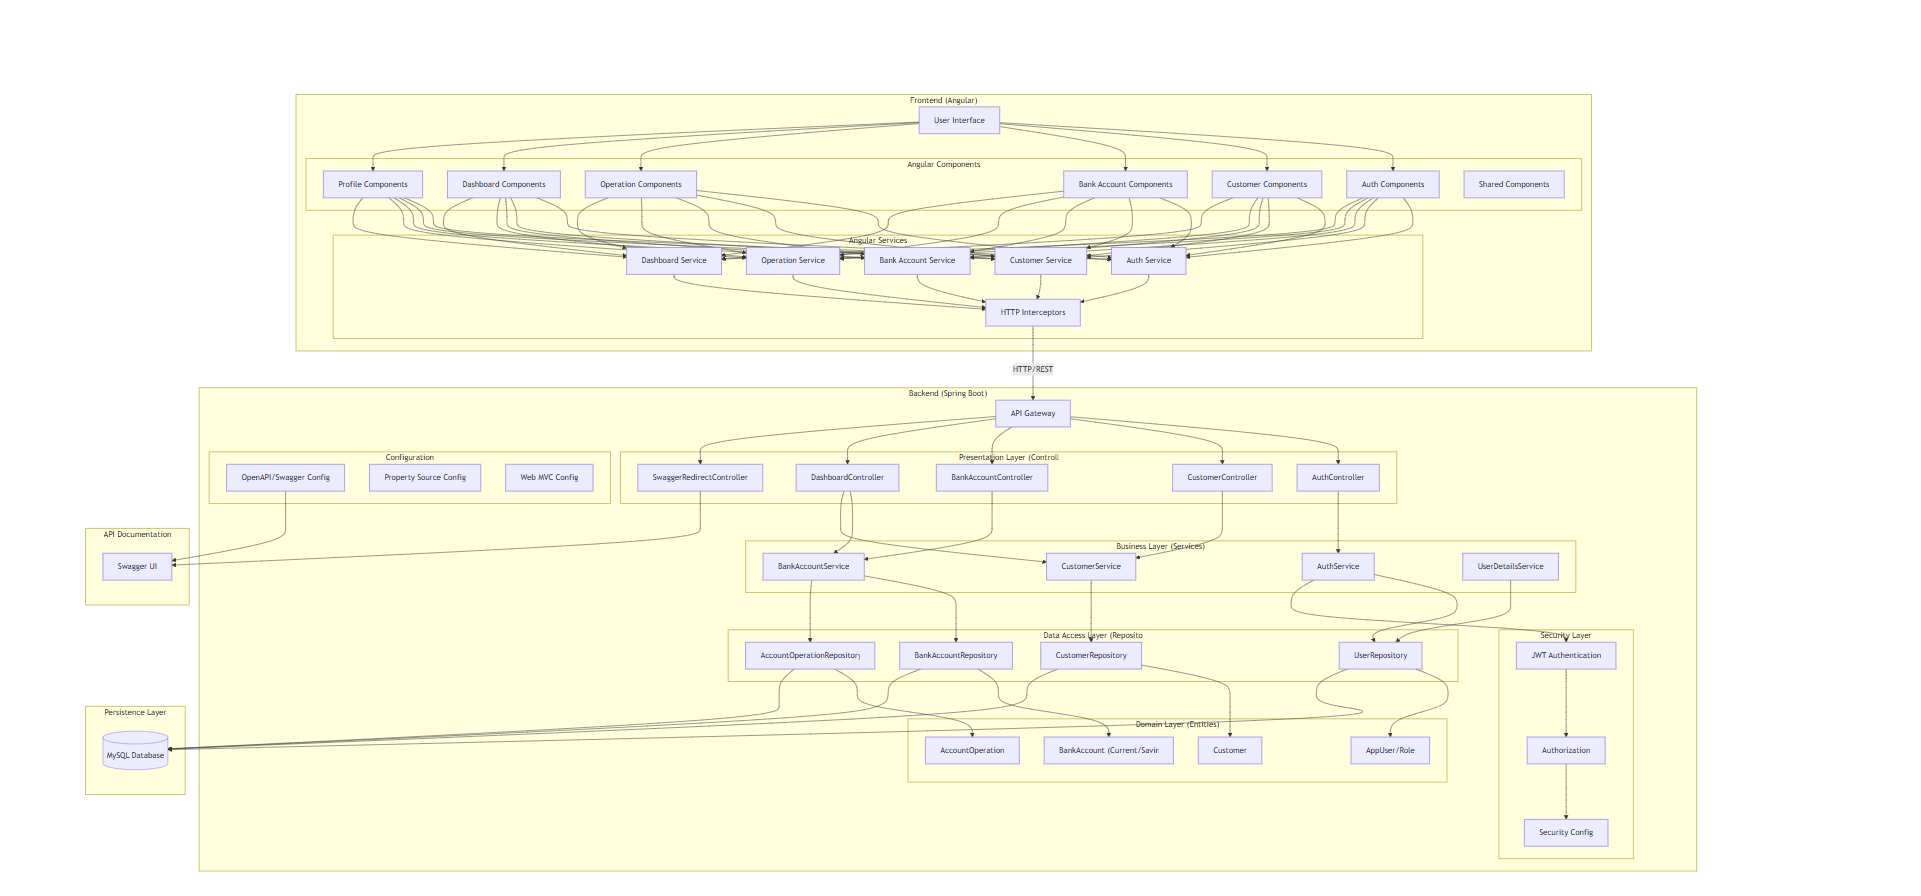
\includegraphics[width=0.98\linewidth]{screenshots/architecture_diagram.png}
    \end{imagebox}
    \caption{\textbf{Diagramme de l'Architecture Générale de l'Application Digital Banking}}
    \label{fig:architecture_diagram}
\end{figure}
\end{landscape}

\subsection{Description Détaillée de l'Architecture}

\begin{infobox}[title=Organisation de l'Architecture]
    L'architecture de Digital Banking est organisée en couches distinctes avec des responsabilités 
    clairement définies, suivant les principes de conception modernes pour assurer la séparation 
    des préoccupations et faciliter la maintenance.
\end{infobox}

\subsubsection{Frontend (Angular)}

\featureheading{Couche Présentation}

\begin{minipage}{\textwidth}
    \begin{minipage}{0.68\textwidth}
        La partie cliente de l'application est développée avec Angular. Elle est responsable de l'interface 
        utilisateur (UI) et de l'expérience utilisateur (UX).
        
        \vspace{0.5cm}
        \begin{secondarybox}[title=Composants Principaux]
            \begin{itemize}[leftmargin=15pt, itemsep=3pt]
                \item \iconbullet{\faUser}{Composants de profil utilisateur}
                \item \iconbullet{\faTachometerAlt}{Composants du tableau de bord}
                \item \iconbullet{\faExchangeAlt}{Composants des opérations bancaires}
                \item \iconbullet{\faPiggyBank}{Composants de gestion des comptes}
                \item \iconbullet{\faUserTie}{Composants de gestion des clients}
                \item \iconbullet{\faLock}{Composants d'authentification}
                \item \iconbullet{\faPuzzlePiece}{Composants partagés réutilisables}
            \end{itemize}
        \end{secondarybox}
    \end{minipage}
    \hfill
    \begin{minipage}{0.28\textwidth}
        \begin{tcolorbox}[
            enhanced,
            colback=primary!5,
            colframe=primary,
            arc=5pt,
            title=Services Angular,
            fonttitle=\small\bfseries\sffamily\color{white},
            coltitle=white,
            colbacktitle=primary
        ]
            \begin{itemize}[leftmargin=12pt, itemsep=2pt, font=\small\sffamily]
                \item DashboardService
                \item OperationService
                \item BankAccountService
                \item CustomerService
                \item AuthService
            \end{itemize}
        \end{tcolorbox}
        
        \vspace{0.5cm}
        
        \begin{tcolorbox}[
            enhanced,
            colback=tertiary!5,
            colframe=tertiary,
            arc=5pt,
            title=Intercepteurs HTTP,
            fonttitle=\small\bfseries\sffamily\color{white},
            coltitle=white,
            colbacktitle=tertiary
        ]
            \begin{itemize}[leftmargin=12pt, itemsep=2pt, font=\small\sffamily]
                \item AuthInterceptor
                \item ErrorInterceptor
            \end{itemize}
        \end{tcolorbox}
    \end{minipage}
\end{minipage}

\vspace{0.8cm}

\subsubsection{Communication (HTTP/REST)}

\begin{tcolorbox}[
    enhanced,
    colback=info!5,
    colframe=info,
    arc=5pt,
    left=8pt,right=8pt,top=8pt,bottom=8pt
]
    \begin{center}
        \faExchangeAlt \quad 
        \textbf{\sffamily\textcolor{info}{Communication RESTful}}
    \end{center}
    
    Le frontend communique avec le backend via des requêtes HTTP, suivant les principes 
    de l'architecture REST (Representational State Transfer). Les données sont échangées au format JSON.
    
    \begin{center}
        \begin{tabular}{|>{\columncolor{info!10}}c|>{\columncolor{white}}c|}
            \hline
            \rowcolor{info!30}
            \textbf{\sffamily\small Méthode HTTP} & \textbf{\sffamily\small Utilisation} \\
            \hline
            \texttt{GET} & Récupération de données \\
            \texttt{POST} & Création de nouvelles ressources \\
            \texttt{PUT} & Mise à jour complète de ressources \\
            \texttt{PATCH} & Mise à jour partielle de ressources \\
            \texttt{DELETE} & Suppression de ressources \\
            \hline
        \end{tabular}
    \end{center}
\end{tcolorbox}

\vspace{0.8cm}

\subsubsection{Backend (Spring Boot)}

\featureheading{Architecture en couches}

\begin{minipage}{\textwidth}
    \begin{minipage}{0.48\textwidth}
        \begin{secondarybox}[title=Couches applicatives]
            \processstep{1}{API Gateway / Présentation (Controllers)}
            \processstep{2}{Logique métier (Services)}
            \processstep{3}{Accès aux données (Repositories)}
            \processstep{4}{Modèle de domaine (Entities)}
        \end{secondarybox}
    \end{minipage}
    \hfill
    \begin{minipage}{0.48\textwidth}
        \begin{tcolorbox}[
            enhanced,
            colback=secondary!5,
            colframe=secondary,
            arc=5pt,
            title=Avantages de cette architecture,
            fonttitle=\small\bfseries\sffamily\color{white},
            coltitle=white,
            colbacktitle=secondary
        ]
            \begin{itemize}[leftmargin=12pt, itemsep=2pt, font=\small\sffamily]
                \item Séparation claire des responsabilités
                \item Testabilité accrue de chaque couche
                \item Facilité de maintenance et d'évolution
                \item Réutilisabilité des composants
                \item Robustesse face aux changements
            \end{itemize}
        \end{tcolorbox}
    \end{minipage}
\end{minipage}

\vspace{0.5cm}

\begin{tcolorbox}[
    enhanced,
    colback=white,
    colframe=bordercolor,
    arc=5pt,
    boxrule=1pt
]
    \begin{center}
        \textbf{\large\sffamily\textcolor{secondary}{Détail des couches backend}}
    \end{center}
    
    \begin{itemize}[leftmargin=20pt, itemsep=5pt]
        \item \textbf{Controllers} : \texttt{DashboardController}, \texttt{BankAccountController}, \texttt{CustomerController}, \texttt{AuthController}, \texttt{SwaggerRedirectController}
        
        \item \textbf{Services} : \texttt{BankAccountService}, \texttt{CustomerService}, \texttt{AuthService}, \texttt{UserDetailsService}
        
        \item \textbf{Repositories} : \texttt{AccountOperationRepository}, \texttt{BankAccountRepository}, \texttt{CustomerRepository}, \texttt{UserRepository}
        
        \item \textbf{Entities} : \texttt{AccountOperation}, \texttt{BankAccount} (avec \texttt{CurrentAccount} et \texttt{SavingAccount}), \texttt{Customer}, \texttt{AppUser}, \texttt{Role}
    \end{itemize}
\end{tcolorbox}

\vspace{0.8cm}

\subsubsection{Persistence Layer}

\begin{secondarybox}[title=Système de persistance]

    \textbf{MySQL Database} est utilisée comme système de gestion de base de données relationnelle 
    pour stocker toutes les données persistantes de l'application :
    \begin{itemize}[leftmargin=15pt, itemsep=2pt]
        \item Informations des clients
        \item Détails des comptes bancaires
        \item Historique des transactions
        \item Utilisateurs et rôles du système
    \end{itemize}
\end{secondarybox}

\vspace{0.8cm}

\subsubsection{Transversal Concerns}

\begin{minipage}{\textwidth}
    \begin{minipage}{0.48\textwidth}
        \begin{tcolorbox}[
            enhanced,
            colback=danger!5,
            colframe=danger,
            arc=5pt,
            title=Sécurité,
            fonttitle=\small\bfseries\sffamily\color{white},
            coltitle=white,
            colbacktitle=danger
        ]
            \begin{itemize}[leftmargin=12pt, itemsep=2pt, font=\small\sffamily]
                \item \textbf{JWT Authentication} : Authentification par jetons
                \item \textbf{Authorization} : Gestion des droits d'accès
                \item \textbf{Security Config} : Règles de sécurité centralisées
            \end{itemize}
        \end{tcolorbox}
    \end{minipage}
    \hfill
    \begin{minipage}{0.48\textwidth}
        \begin{tcolorbox}[
            enhanced,
            colback=info!5,
            colframe=info,
            arc=5pt,
            title=Documentation API,
            fonttitle=\small\bfseries\sffamily\color{white},
            coltitle=white,
            colbacktitle=info
        ]
            \begin{itemize}[leftmargin=12pt, itemsep=2pt, font=\small\sffamily]
                \item \textbf{Swagger UI} : Interface d'exploration de l'API
                \item \textbf{OpenAPI} : Spécification standardisée
                \item \textbf{Annotations} : Documentation intégrée au code
            \end{itemize}
        \end{tcolorbox}
    \end{minipage}
\end{minipage}

\vspace{0.5cm}

\technote{
    Cette architecture multicouche favorise le découplage, la testabilité et la clarté du code, 
    des aspects essentiels pour le développement et la maintenance d'une application complexe 
    comme Digital Banking.
}

\keypoint{
    En résumé, l'architecture de Digital Banking illustre une application moderne, 
    tirant parti des meilleures pratiques pour créer un système bancaire numérique 
    robuste, sécurisé et maintenable.
}

% --- END OF ARCHITECTURE SECTION ---
\clearpage % Ensure content after landscape starts on a new page in portrait

\section{Authentification}

\sectiondivider

\begin{warningbox}[title=Sécurité renforcée]
    L'accès à l'application est protégé par un système d'authentification robuste 
    basé sur JSON Web Tokens (JWT), garantissant que seuls les utilisateurs 
    autorisés peuvent accéder aux fonctionnalités bancaires.
    
    \iconbullet{\faShieldAlt}{Protection contre les attaques par force brute}
    \iconbullet{\faKey}{Gestion sécurisée des sessions utilisateur}
    \iconbullet{\faUserLock}{Contrôle d'accès basé sur les rôles}
\end{warningbox}

\subsection{Page de Connexion Initiale}

\featureshowcase{Interface d'authentification}{
    Au lancement de l'application, l'utilisateur est accueilli par une interface de connexion 
    épurée et professionnelle. Cette page constitue le point d'entrée sécurisé vers l'ensemble 
    des fonctionnalités bancaires.
    
    \vspace{0.3cm}
    \iconbullet{\faUser}{Champ pour identifiant unique}
    \iconbullet{\faLock}{Champ de mot de passe masqué}
    \iconbullet{\faSignInAlt}{Bouton de connexion intuitif}
}{screenshots/01_01_login_page_initial.png}

\vspace{0.5cm}

\begin{center}
    \begin{tikzpicture}
        \node[draw=primary, thick, rounded corners, fill=primary!5, text width=0.8\textwidth, inner sep=10pt] {
            \centering
            \textbf{\sffamily\textcolor{primary}{Flux d'authentification sécurisé}}\\
            \begin{tikzpicture}
                \draw[->, thick, primary] (0,0) -- (1,0) node[midway, above, font=\small\sffamily] {1};
                \node[right, text width=3cm, align=left, font=\small\sffamily] at (1,0) {Saisie des identifiants};
                
                \draw[->, thick, primary] (4,0) -- (5,0) node[midway, above, font=\small\sffamily] {2};
                \node[right, text width=3cm, align=left, font=\small\sffamily] at (5,0) {Validation serveur};
                
                \draw[->, thick, primary] (8,0) -- (9,0) node[midway, above, font=\small\sffamily] {3};
                \node[right, text width=3cm, align=left, font=\small\sffamily] at (9,0) {Génération JWT};
            \end{tikzpicture}
        };
    \end{tikzpicture}
\end{center}

\apiendpoint{POST}{/api/auth/login}{
    Endpoint d'authentification qui valide les identifiants et génère un JWT
}{
    \{token: "eyJhbGciOiJIUzI1...", username: "admin\_user", roles: ["ADMIN"]\}
}

\subsection{Gestion des Erreurs d'Authentification}

\begin{minipage}{\textwidth}
    \begin{minipage}{0.58\textwidth}
        \begin{secondarybox}[title=Mécanisme de sécurité proactif]
            Le système intègre une gestion d'erreurs claire et informative. Lorsque des identifiants 
            incorrects sont saisis, un message d'erreur explicite guide l'utilisateur sans compromettre 
            la sécurité du système.
            
            \vspace{0.3cm}
            Les techniques implémentées incluent:
            \begin{itemize}[leftmargin=15pt, itemsep=2pt]
                \item Messages d'erreur génériques ne révélant pas d'informations sensibles
                \item Temporisation pour contrer les attaques par force brute
                \item Journalisation des tentatives d'accès échouées
            \end{itemize}
        \end{secondarybox}
    \end{minipage}
    \hfill
    \begin{minipage}{0.38\textwidth}
        \begin{imagebox}
            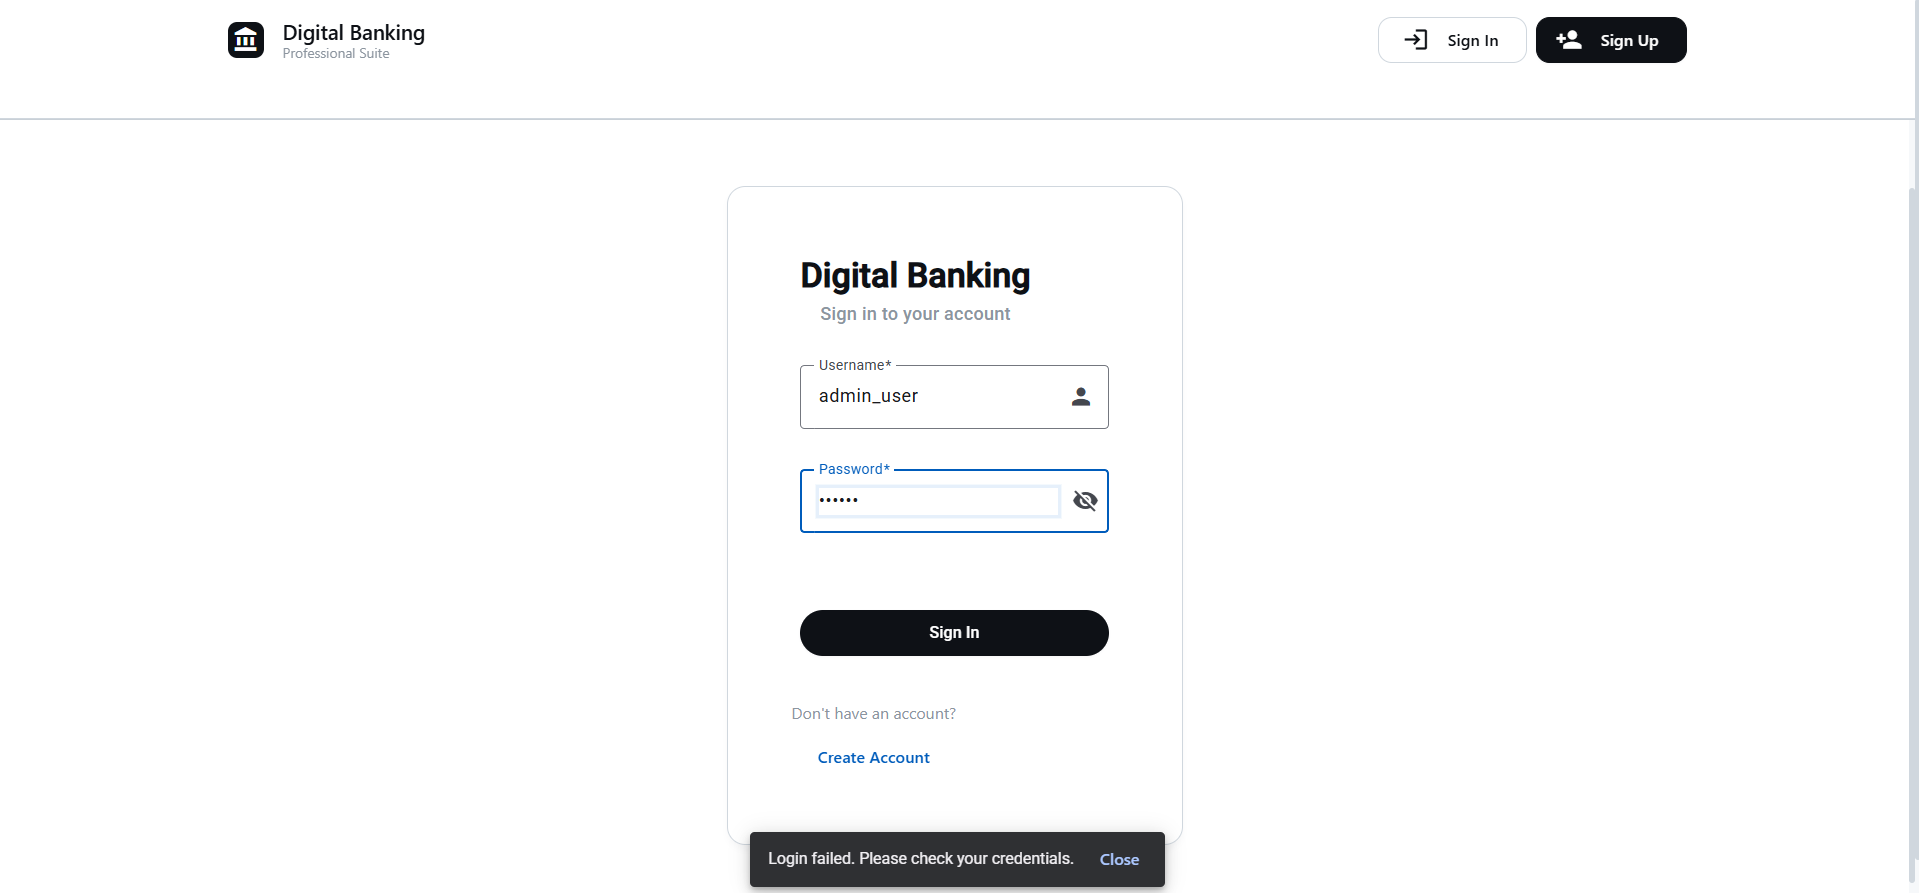
\includegraphics[width=\textwidth]{screenshots/01_02_login_page_incorrect_credentials.png}
            \caption*{\textbf{\sffamily\small Message d'erreur informatif}}
        \end{imagebox}
    \end{minipage}
\end{minipage}

\vspace{0.8cm}

\subsection{Accès Réussi au Tableau de Bord}

\begin{infobox}[title=Authentification réussie]
    Après une authentification réussie avec les identifiants valides (\texttt{admin\_user} / \texttt{123456}), 
    l'utilisateur est automatiquement redirigé vers le tableau de bord principal, offrant une vue 
    d'ensemble immédiate de son espace bancaire.
\end{infobox}

\begin{figure}[h]
    \centering
    \vspace{1cm}
    \begin{imagebox}
        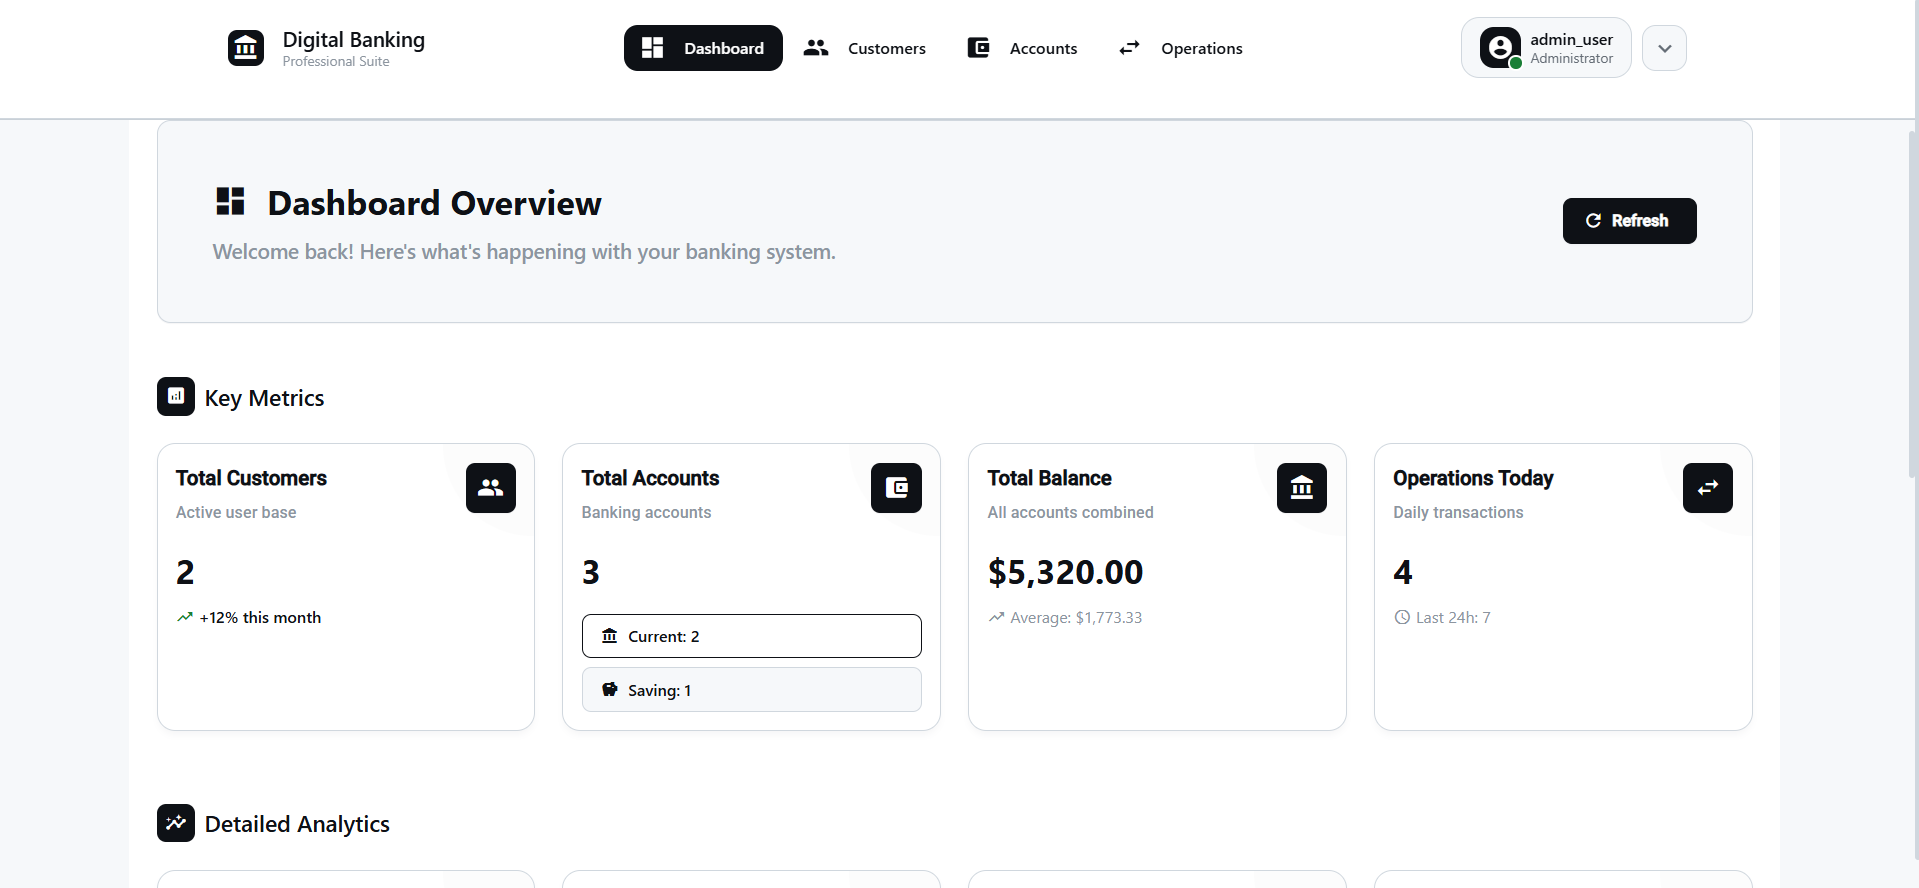
\includegraphics[width=0.95\textwidth]{screenshots/01_03_login_successful_dashboard.png}
    \end{imagebox}
    \caption{\textbf{Redirection post-authentification} - Accès direct au tableau de bord personnalisé}
    \label{fig:login_successful}
    \vspace{0.8cm}
\end{figure}

\technote{
    Le système d'authentification utilise Spring Security côté backend et des intercepteurs HTTP côté frontend 
    pour garantir que chaque requête est accompagnée du JWT valide. Cette approche sans état (stateless) 
    permet une meilleure scalabilité de l'application.
}

\newpage


\section{Tableau de Bord}

\sectiondivider

\begin{successbox}[title=Centre de contrôle utilisateur]
    Le tableau de bord constitue le centre névralgique de l'application, offrant une vue 
    synthétique et interactive des données financières de l'utilisateur. Il permet une 
    prise de décision éclairée grâce à la visualisation immédiate des informations importantes.
\end{successbox}

\subsection{Vue d'Ensemble Interactive}

\begin{minipage}{\textwidth}
    \begin{minipage}{0.35\textwidth}
        \begin{tcolorbox}[
            enhanced,
            colback=secondary!5,
            colframe=secondary,
            arc=5pt,
            title=Fonctionnalités clés,
            fonttitle=\small\bfseries\sffamily\color{white},
            coltitle=white,
            colbacktitle=secondary
        ]
            \begin{itemize}[leftmargin=15pt, itemsep=3pt, font=\small\sffamily]
                \item \textbf{Distribution des comptes} par type
                \item \textbf{Tendances des opérations} financières
                \item \textbf{Indicateurs en temps réel} sur l'activité
                \item \textbf{Navigation intuitive} entre les sections
                \item \textbf{Résumé des dernières opérations}
            \end{itemize}
        \end{tcolorbox}
        
        \vspace{0.5cm}
        
        \begin{tikzpicture}
            \node[draw=success, thick, rounded corners, fill=success!5, text width=\textwidth, inner sep=10pt] {
                \centering
                \textbf{\sffamily\textcolor{success}{Avantages}}\\
                \vspace{0.2cm}
                \iconbullet{\faChartPie}{Visualisation immédiate des données}
                \iconbullet{\faRocket}{Accès rapide aux fonctionnalités}
                \iconbullet{\faSearch}{Vision globale de l'activité}
                \iconbullet{\faBell}{Alertes et notifications importantes}
            };
        \end{tikzpicture}
    \end{minipage}
    \hfill
    \begin{minipage}{0.62\textwidth}
        \begin{imagebox}
            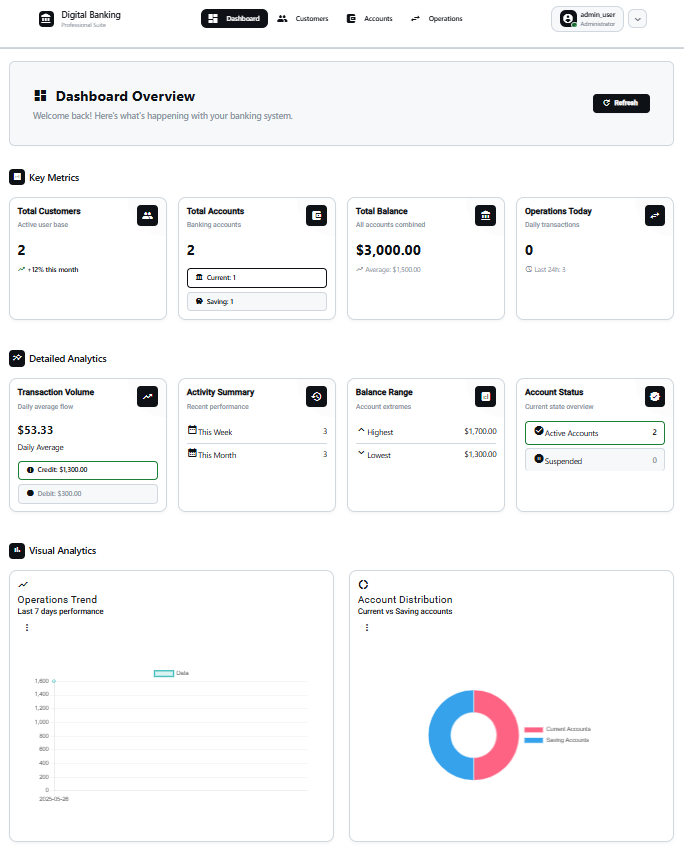
\includegraphics[width=\textwidth]{screenshots/02_01_dashboard_overview.png}
            \caption*{\textbf{\sffamily Interface centralisée avec graphiques interactifs}}
        \end{imagebox}
    \end{minipage}
\end{minipage}

\vspace{0.8cm}

\begin{tcolorbox}[
    enhanced,
    colback=primary!5,
    colframe=primary,
    arc=5pt,
    left=10pt,right=10pt,top=10pt,bottom=10pt
]
    \begin{center}
        \textbf{\large\sffamily\textcolor{primary}{Architecture des composants du tableau de bord}}
    \end{center}
    
    \begin{tikzpicture}[
        node distance=1.5cm,
        box/.style={draw=primary, thick, fill=white, minimum width=3cm, minimum height=1cm, rounded corners, font=\sffamily}
    ]
        \node[box] (dash) {\textbf{DashboardComponent}};
        \node[box, below left=of dash] (charts) {ChartComponents};
        \node[box, below=of dash] (summary) {SummaryComponent};
        \node[box, below right=of dash] (nav) {NavigationComponent};
        
        \draw[->, thick, primary] (dash) -- (charts);
        \draw[->, thick, primary] (dash) -- (summary);
        \draw[->, thick, primary] (dash) -- (nav);
    \end{tikzpicture}
\end{tcolorbox}

\technote{
    Les graphiques du tableau de bord sont générés dynamiquement à partir des données récupérées 
    via l'API REST. La bibliothèque Chart.js est utilisée pour le rendu des visualisations, 
    offrant une expérience interactive et réactive aux utilisateurs.
}

\section{Gestion des Clients}

\sectiondivider

\begin{primarybox}[title=Module de gestion clientèle]
    Ce module complet est dédié à l'administration des profils clients avec fonctionnalités 
    CRUD (Créer, Lire, Mettre à jour, Supprimer) intégrées dans une interface intuitive et réactive.
    
    La gestion des clients est un élément central de l'application, permettant aux administrateurs 
    de maintenir une base de données à jour et d'assurer la qualité des informations utilisées 
    pour toutes les opérations bancaires.
\end{primarybox}

\subsection{Consultation de la Base Clients}

\begin{minipage}{\textwidth}
    \begin{minipage}{0.32\textwidth}
        \begin{tcolorbox}[
            enhanced,
            colback=tertiary!5,
            colframe=tertiary,
            arc=5pt,
            title=Fonctionnalités de consultation,
            fonttitle=\small\bfseries\sffamily\color{white},
            coltitle=white,
            colbacktitle=tertiary
        ]
            \begin{itemize}[leftmargin=12pt, itemsep=3pt, font=\small\sffamily]
                \item \textbf{Recherche} par nom ou identifiant
                \item \textbf{Pagination} pour navigation efficace
                \item \textbf{Tri} par colonnes multiples
                \item \textbf{Actions rapides} sur chaque ligne
                \item \textbf{Vue responsive} adaptable
            \end{itemize}
        \end{tcolorbox}
    \end{minipage}
    \hfill
    \begin{minipage}{0.65\textwidth}
        \begin{imagebox}
            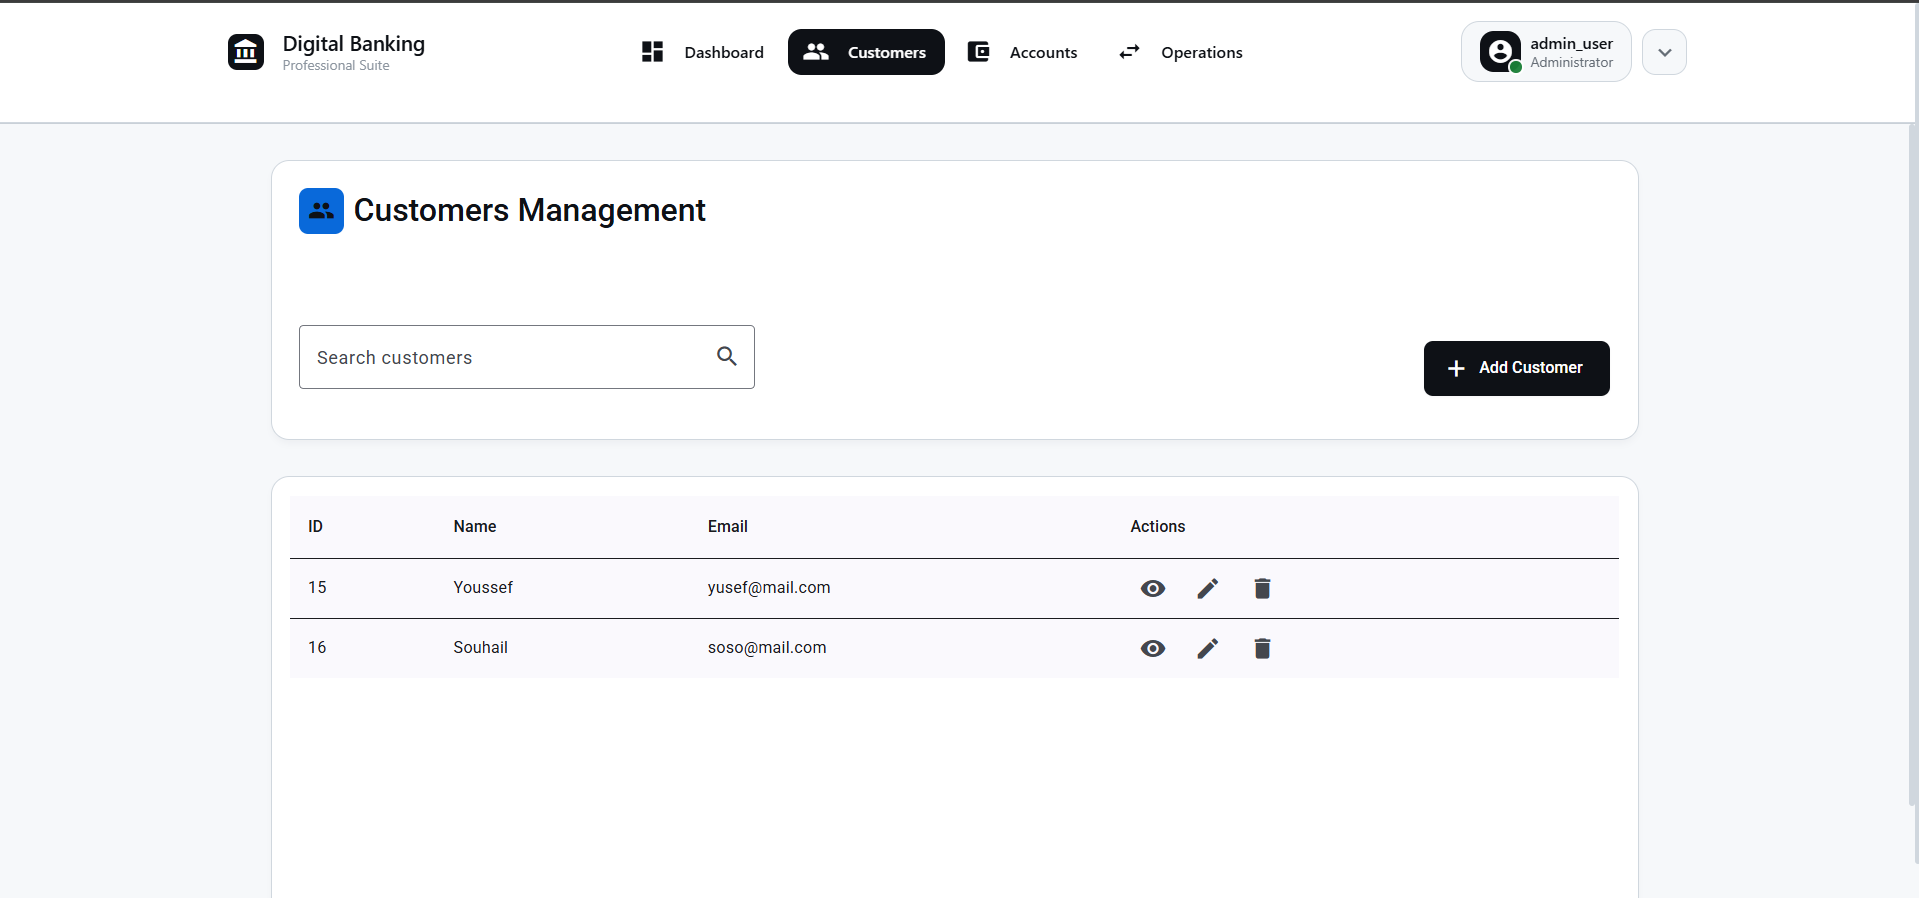
\includegraphics[width=\textwidth]{screenshots/04_01_customer_list_initial.png}
            \caption*{\textbf{\sffamily Interface de gestion des clients}}
        \end{imagebox}
    \end{minipage}
\end{minipage}

\apiendpoint{GET}{/api/customers}{
    Récupère la liste paginée des clients avec options de tri et filtrage
}{
    \{"customers": [...], "totalPages": 5, "currentPage": 0, "totalItems": 42\}
}

\vspace{0.8cm}

\subsection{Création de Nouveaux Profils}

\begin{infobox}[title=Processus de création de client]
    L'ajout de nouveaux clients s'effectue via un formulaire intuitif qui guide l'utilisateur 
    à travers la saisie de toutes les informations nécessaires. La validation en temps réel 
    garantit l'intégrité des données avant leur soumission.
\end{infobox}

\begin{minipage}{\textwidth}
    \begin{minipage}{0.48\textwidth}
        \subsubsection{Formulaire de Saisie}
        \begin{imagebox}
            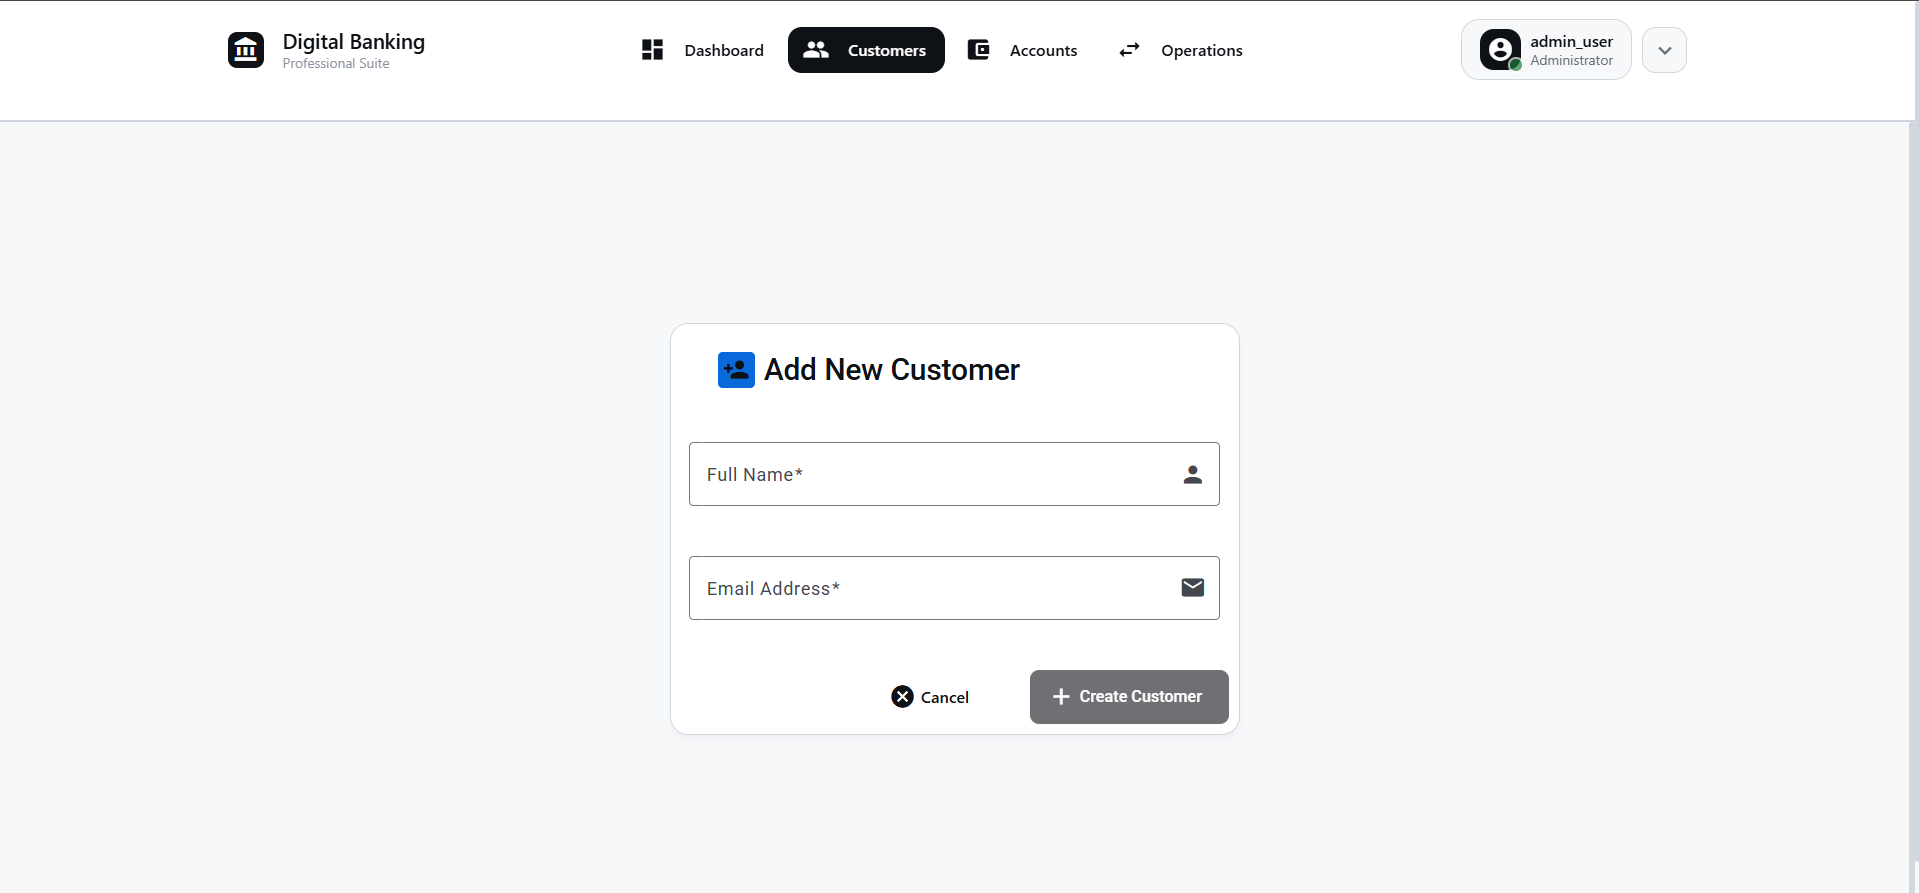
\includegraphics[width=\textwidth]{screenshots/04_02_customer_form_new_empty.png}
            \caption*{\textbf{\sffamily\small Formulaire vierge}}
        \end{imagebox}
    \end{minipage}
    \hfill
    \begin{minipage}{0.48\textwidth}
        \subsubsection{Formulaire Complété}
        \begin{imagebox}
            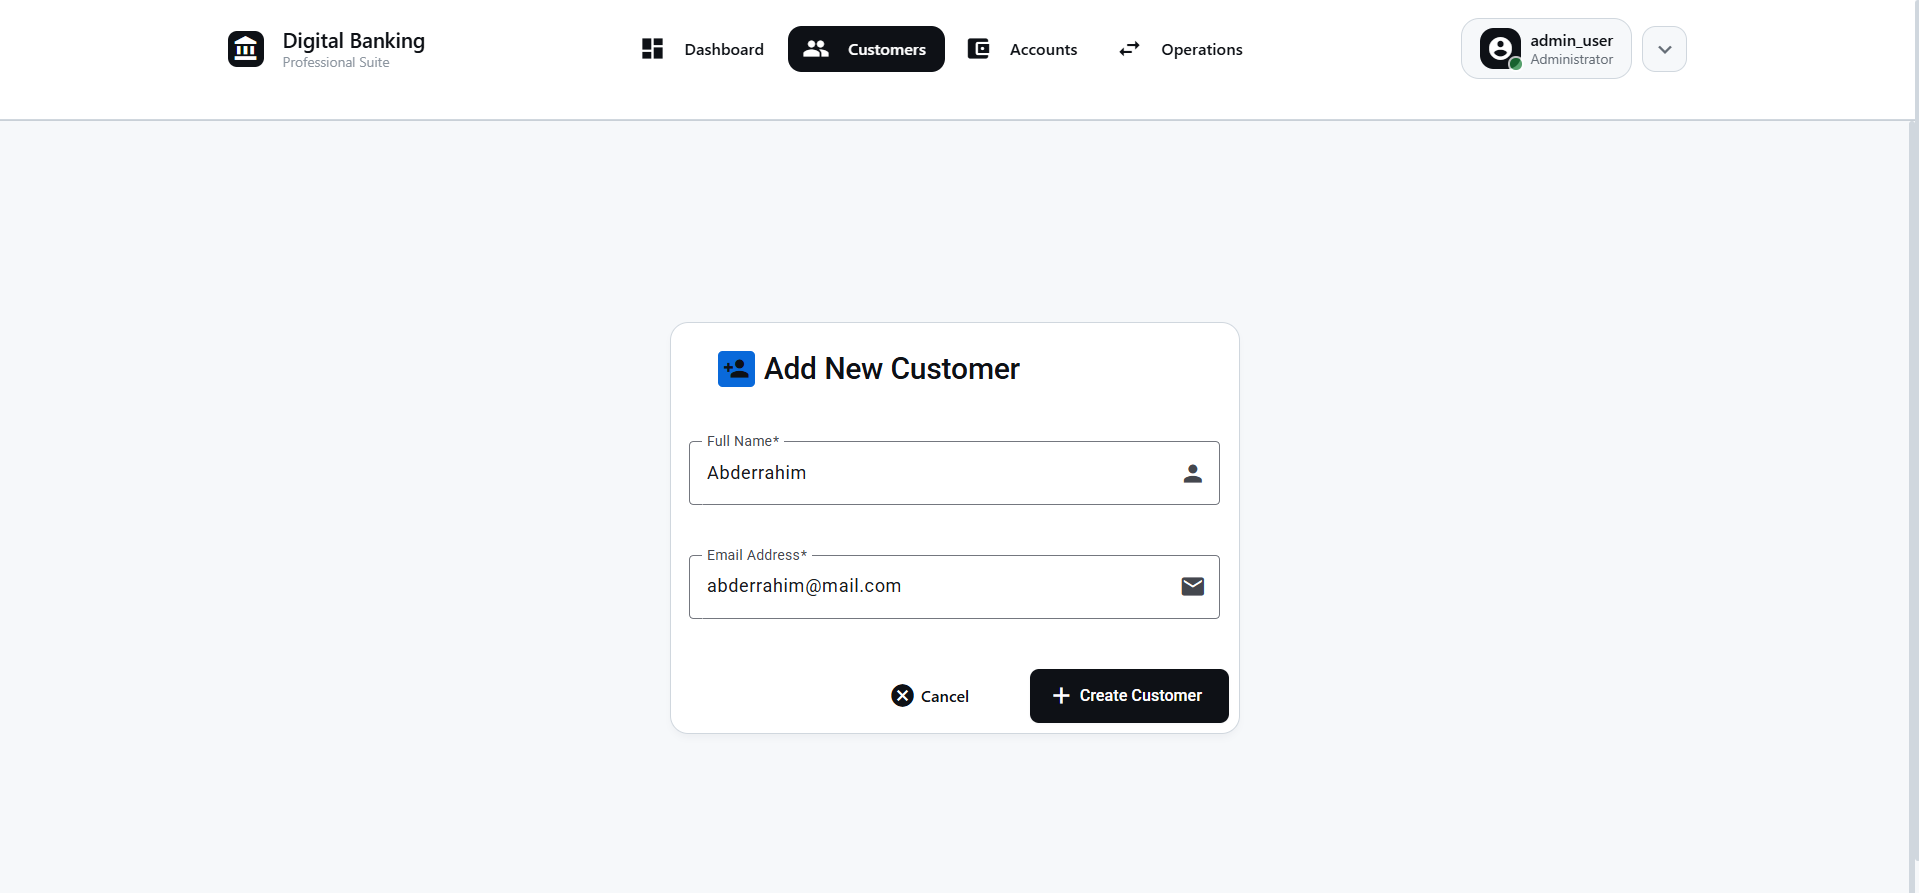
\includegraphics[width=\textwidth]{screenshots/04_03_customer_form_new_filled.png}
            \caption*{\textbf{\sffamily\small Exemple de saisie}}
        \end{imagebox}
    \end{minipage}
\end{minipage}

\vspace{0.8cm}

\codesnippet{Modèle Angular du Client}{
export class Customer \{
  id: string;
  name: string;
  email: string;
  phoneNumber?: string;
  address?: string;
  createdAt: Date;
  
  // Relations
  accounts?: BankAccount[];
\}
}

\vspace{0.5cm}

\technote{
    La création de client utilise une approche réactive avec validation côté client et côté serveur. 
    La requête est envoyée via une requête POST au backend, qui valide les données avant de les persister 
    dans la base de données. Une réponse de confirmation avec l'ID généré est retournée au frontend.
}

\subsection{Modification et Suppression de Clients}

\begin{minipage}{\textwidth}
    \begin{minipage}{0.58\textwidth}
        \begin{secondarybox}[title=Cycle de vie complet des clients]
            L'application offre un cycle de vie complet pour la gestion des clients, 
            incluant non seulement la création mais aussi la modification des informations 
            existantes et la suppression lorsque nécessaire.
            
            \vspace{0.3cm}
            \timelineentry{1}{Sélection du client à modifier}{secondary}
            \timelineentry{2}{Formulaire pré-rempli avec données existantes}{secondary}
            \timelineentry{3}{Modification des champs nécessaires}{secondary}
            \timelineentry{4}{Validation et enregistrement des changements}{secondary}
        \end{secondarybox}
    \end{minipage}
    \hfill
    \begin{minipage}{0.38\textwidth}
        \begin{imagebox}
            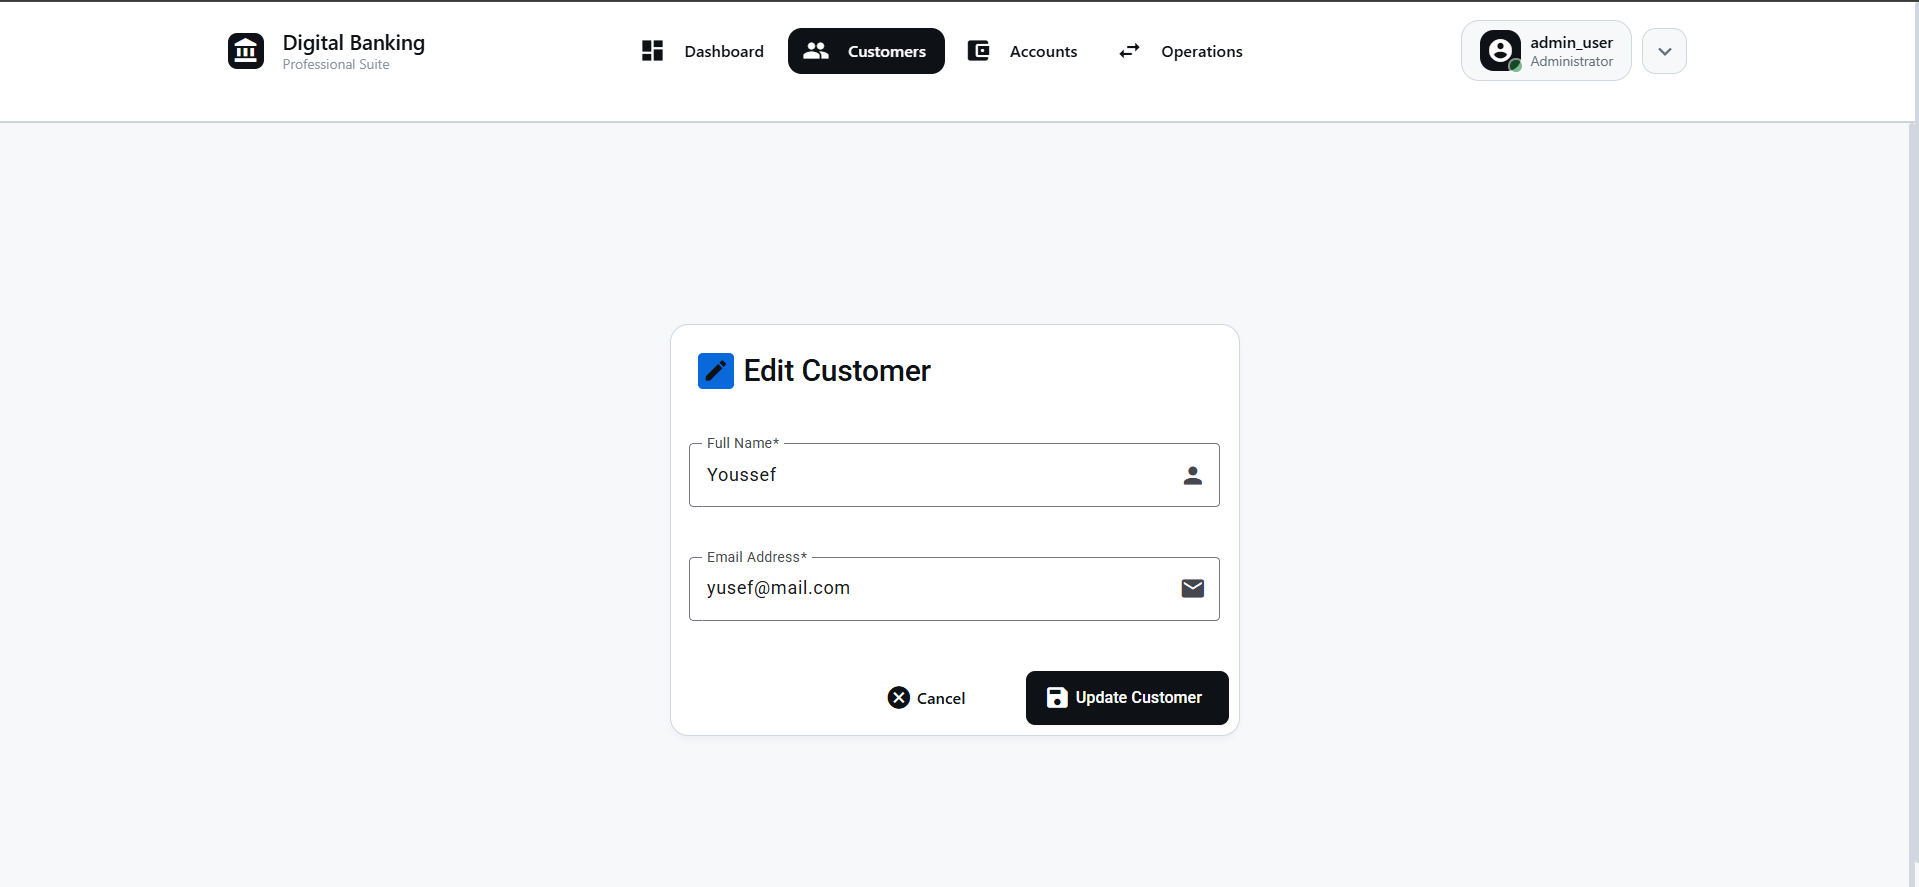
\includegraphics[width=\textwidth]{screenshots/04_05_customer_form_edit_prefilled.png}
            \caption*{\textbf{\sffamily\small Formulaire de modification}}
        \end{imagebox}
        
        \vspace{0.5cm}
        
        \begin{imagebox}
            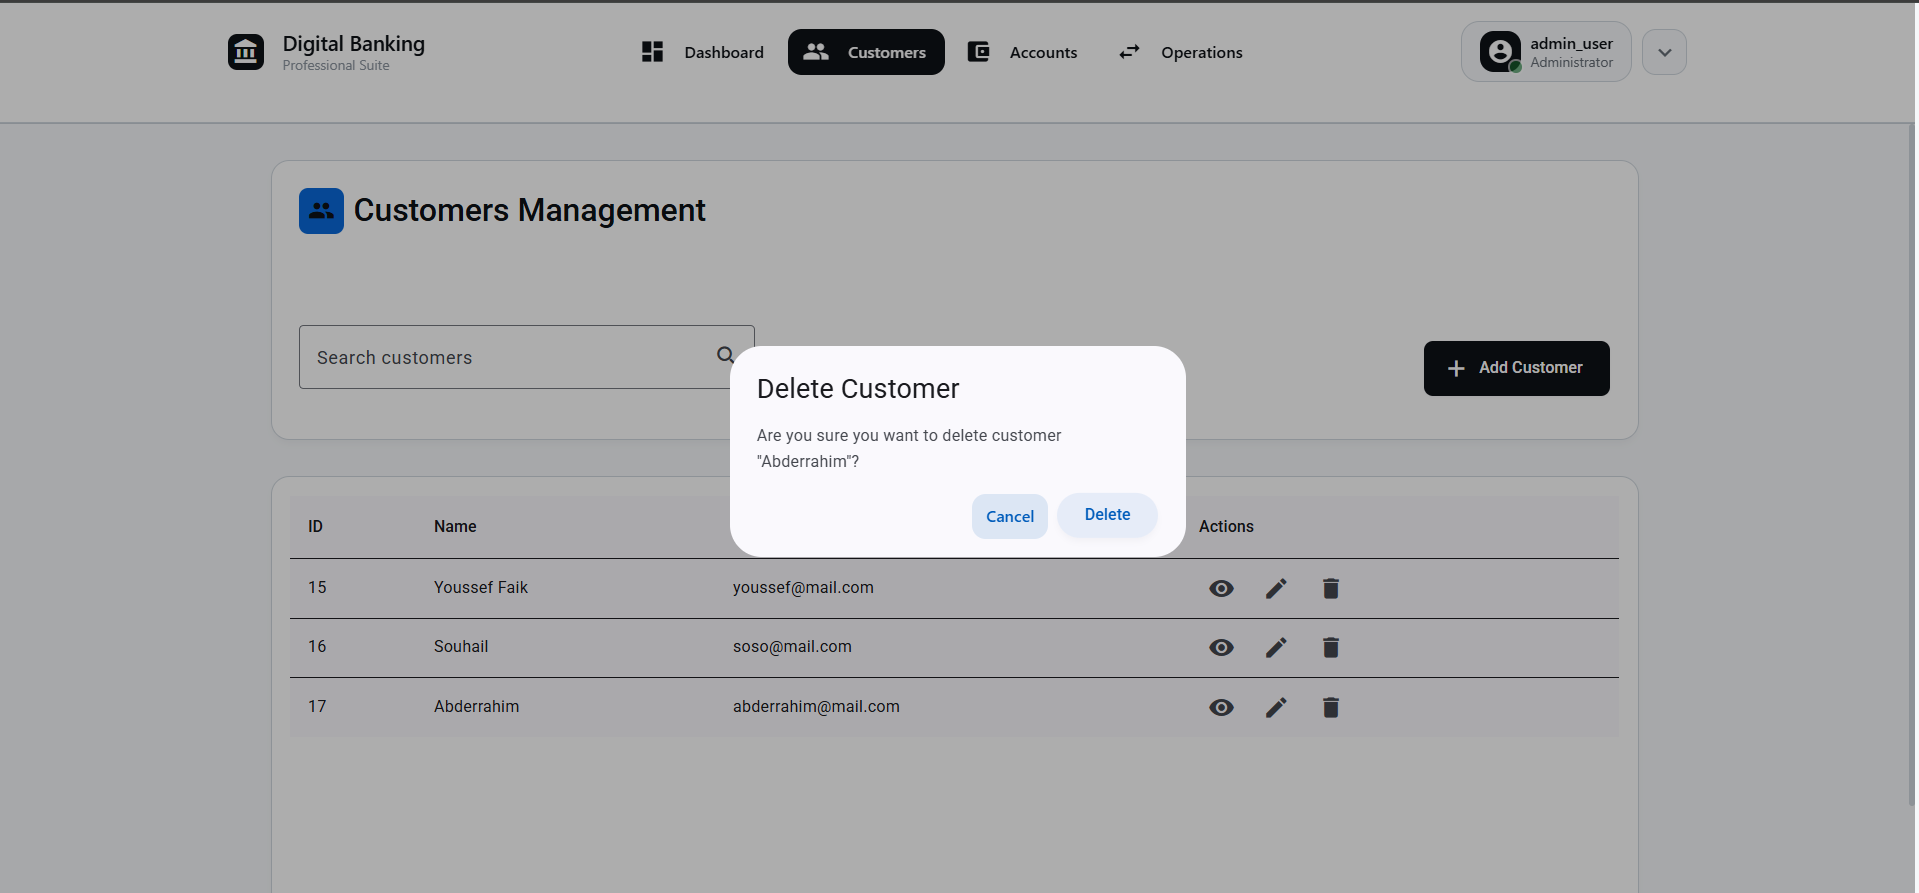
\includegraphics[width=\textwidth]{screenshots/04_08_customer_list_after_delete.png}
            \caption*{\textbf{\sffamily\small Après suppression}}
        \end{imagebox}
    \end{minipage}
\end{minipage}

\vspace{0.8cm}

\begin{tcolorbox}[
    enhanced,
    colback=danger!5,
    colframe=danger,
    arc=5pt,
    left=10pt,right=10pt,top=10pt,bottom=10pt
]
    \begin{center}
        \textbf{\large\sffamily\textcolor{danger}{Précautions pour la suppression de clients}}
    \end{center}
    
    \begin{itemize}[leftmargin=15pt, itemsep=5pt]
        \item \textbf{Confirmation obligatoire} avant toute suppression définitive
        \item \textbf{Vérification des comptes associés} pour éviter les suppressions problématiques
        \item \textbf{Journalisation des suppressions} pour maintenir un audit trail complet
        \item \textbf{Accès restreint} à cette fonctionnalité critique selon les rôles utilisateurs
    \end{itemize}
\end{tcolorbox}

\apiendpoint{DELETE}{/api/customers/\{id\}}{
    Supprime un client après vérification des dépendances et contraintes
}{
    \{"status": "SUCCESS", "message": "Customer deleted successfully"\}
}

\vspace{0.5cm}

\keypoint{
    La gestion complète des clients constitue la fondation de l'application Digital Banking, 
    permettant aux administrateurs de maintenir une base de données clients fiable et à jour.
}

\newpage

% --- SECTION FOR SWAGGER DOCUMENTATION ---
\section{Documentation API avec Swagger}

\begin{tcolorbox}[
    colback=lightgray,
    colframe=primaryblue, 
    boxrule=1pt,
    arc=5pt,
    left=10pt,
    right=10pt,
    top=10pt,
    bottom=10pt
]
\textbf{Transparence et Interactivité :} Pour faciliter la compréhension, l'intégration et le test de l'API backend, une documentation interactive est fournie grâce à Swagger (conforme à la spécification OpenAPI). Elle permet aux développeurs de visualiser l'ensemble des endpoints, de comprendre les modèles de données (schémas) et même de tester les requêtes directement depuis une interface web.
\end{tcolorbox}

\subsection{Vue Générale de Swagger UI}
L'interface Swagger UI offre une vue d'ensemble claire et structurée de toutes les ressources de l'API. Les endpoints sont regroupés par contrôleurs (ou tags), facilitant la navigation et la découverte des fonctionnalités disponibles. Chaque endpoint est listé avec sa méthode HTTP (GET, POST, PUT, DELETE) et un résumé de son objectif.

\begin{figure}[H]
    \centering
    \begin{tcolorbox}[
        width=0.9\textwidth,
        colback=white,
        colframe=secondarygreen, 
        boxrule=1pt,
        arc=5pt,
        boxsep=5pt
    ]
        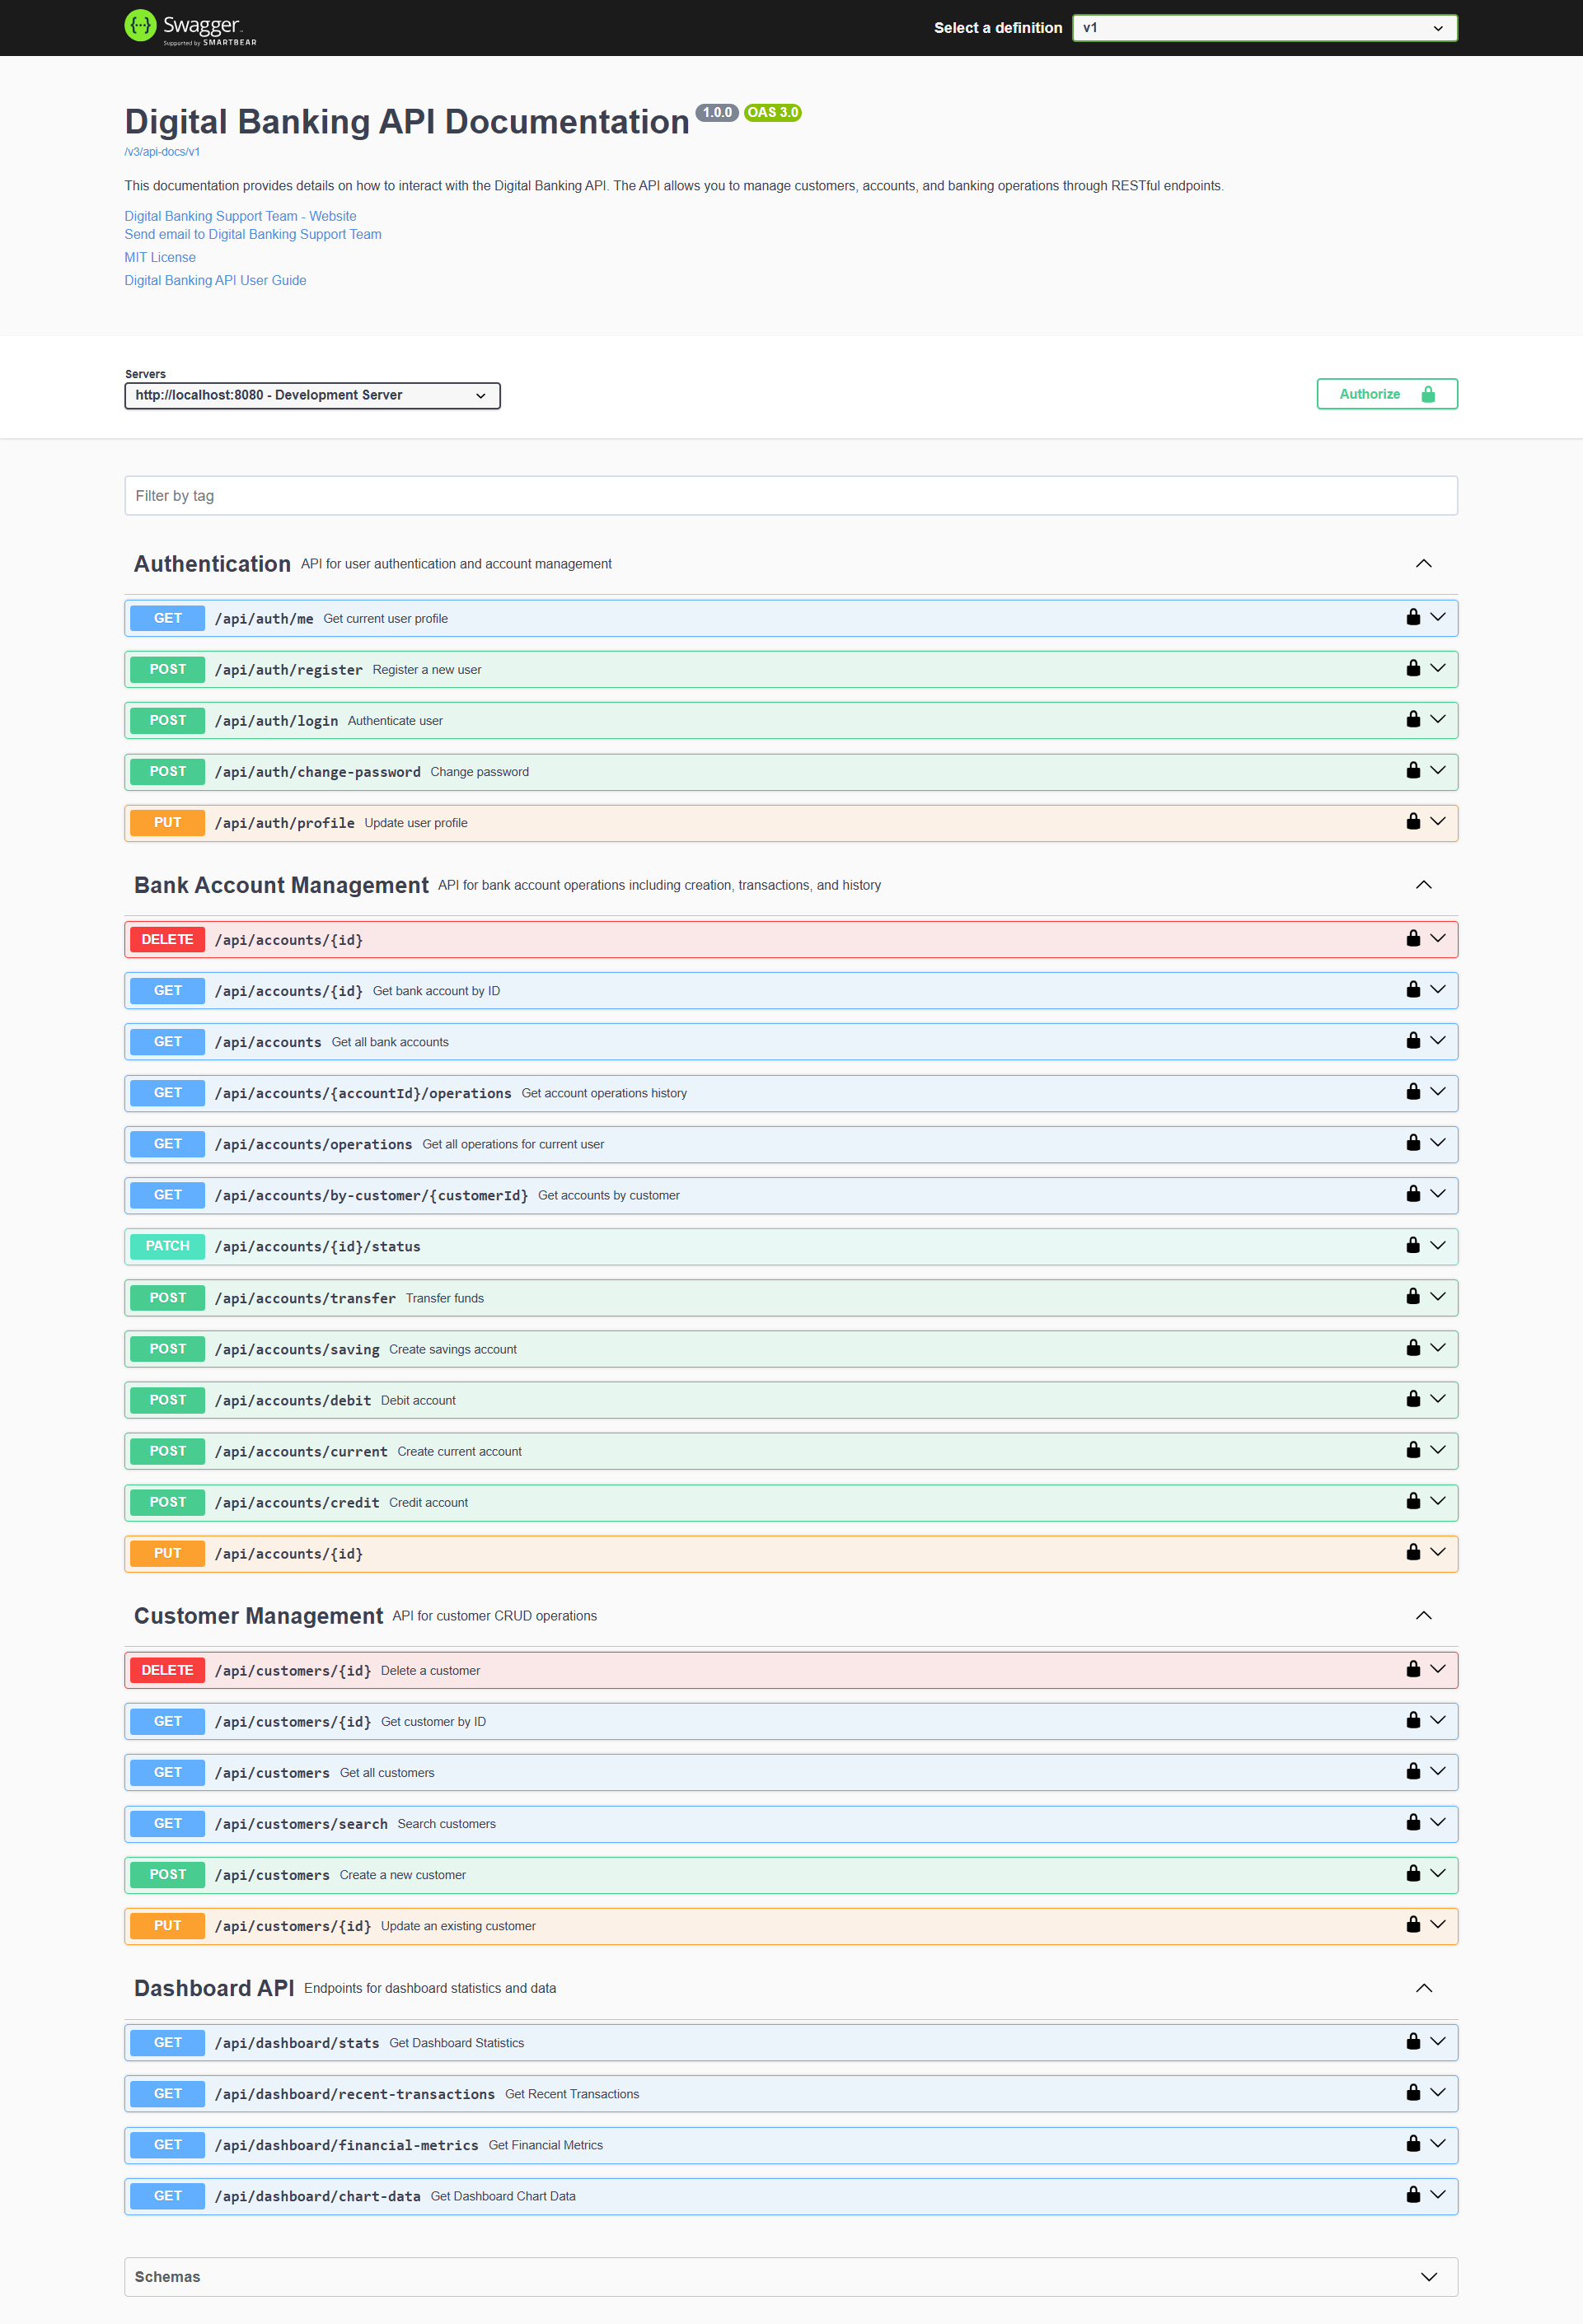
\includegraphics[width=\textwidth]{screenshots/swagger_ui_main.png} 
    \end{tcolorbox}
    \caption{\textbf{Interface principale de Swagger UI} - Liste des contrôleurs et endpoints de l'API}
    \label{fig:swagger_ui_main}
\end{figure}

\subsection{Exploration et Test des Endpoints}
En sélectionnant un endpoint spécifique, l'utilisateur peut accéder à une documentation détaillée incluant la description de la fonctionnalité, les paramètres requis et optionnels (path, query, body), les schémas des corps de requête et de réponse, ainsi que les codes de statut HTTP possibles. La fonctionnalité "Try it out" permet d'exécuter l'endpoint directement depuis l'interface. Ci-dessous, quelques exemples illustratifs :

\paragraph{Exemple 1 : Endpoint d'Authentification}
L'authentification est gérée via un endpoint dédié, typiquement une requête POST vers un chemin comme \texttt{/api/auth/login}. L'utilisateur fournit ses identifiants (nom d'utilisateur et mot de passe) dans le corps de la requête. En retour, l'API délivre un jeton (par exemple, JWT) qui sera utilisé pour autoriser les requêtes subséquentes.

\begin{figure}[H]
    \centering
    \begin{tcolorbox}[
        width=0.9\textwidth,
        colback=white,
        colframe=secondarygreen,
        boxrule=1pt,
        arc=5pt,
        boxsep=5pt
    ]
        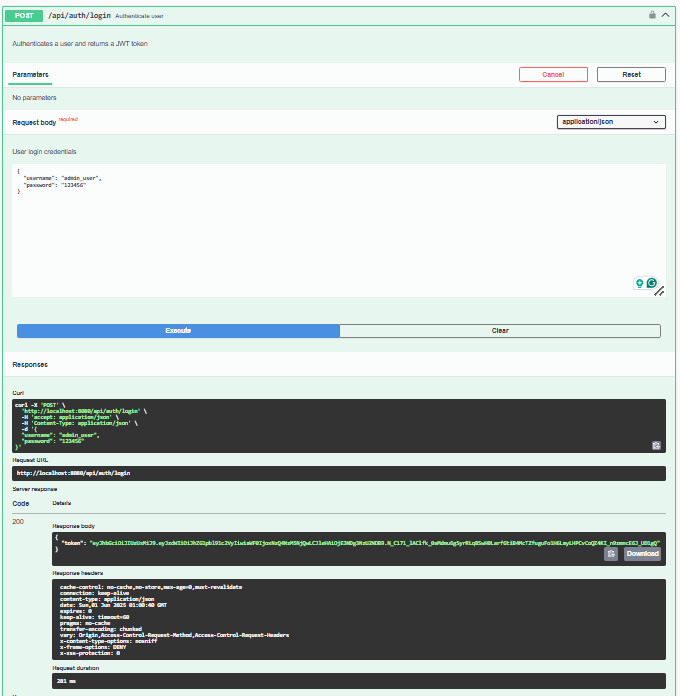
\includegraphics[width=\textwidth]{screenshots/swagger_auth_endpoint.png}
    \end{tcolorbox}
    \caption{\textbf{Exemple d'endpoint d'authentification (POST)} - Paramètres de requête (identifiants) et description de la réponse (jeton d'accès)}
    \label{fig:swagger_auth_endpoint}
\end{figure}

\paragraph{Exemple 2 : Endpoint de Récupération de Données (GET)}
Pour récupérer des informations spécifiques, comme les détails d'un client, un endpoint GET utilisant un paramètre de chemin (path parameter) est souvent utilisé, par exemple \texttt{/api/customers/\{customerId\}}. Swagger UI permet de spécifier la valeur de \texttt{customerId} pour tester l'appel.

\begin{figure}[H]
    \centering
    \begin{tcolorbox}[
        width=0.9\textwidth,
        colback=white,
        colframe=secondarygreen,
        boxrule=1pt,
        arc=5pt,
        boxsep=5pt
    ]
        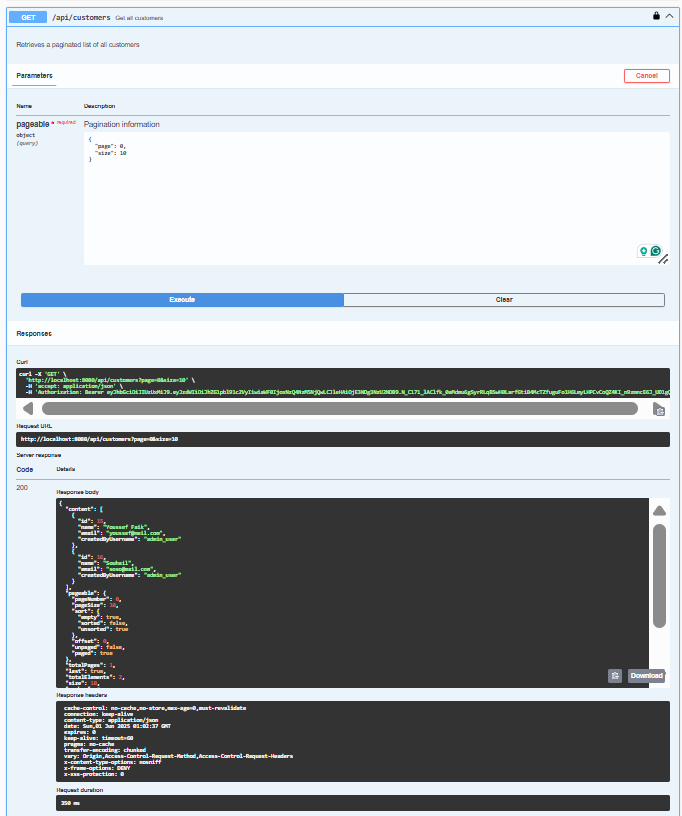
\includegraphics[width=\textwidth]{screenshots/swagger_get_data_endpoint.png}
    \end{tcolorbox}
    \caption{\textbf{Exemple d'endpoint de récupération de données (GET)} - Utilisation d'un paramètre de chemin et visualisation du schéma de réponse}
    \label{fig:swagger_get_data_endpoint}
\end{figure}


L'intégration de Swagger améliore significativement la maintenabilité et la facilité d'utilisation de l'API, en fournissant une source de vérité unique et toujours à jour pour sa documentation.

\newpage

% --- END OF SWAGGER SECTION ---
\section{Conclusion}

\sectiondivider

\begin{primarybox}[title=Synthèse du Projet]
    \begin{center}
        \begin{tabular}{c}
            \textbf{\large\sffamily Une Solution Bancaire Digitale Complète}
        \end{tabular}
    \end{center}
    
    L'application \textbf{Digital Banking} représente un écosystème bancaire numérique complet et moderne, 
    basé sur une architecture robuste et bien structurée, comme détaillé dans ce rapport. 
    
    Elle démontre l'efficacité des technologies contemporaines (\faAngular~Angular, \faJava~Spring Boot) 
    pour créer une expérience utilisateur fluide et sécurisée. La documentation exhaustive des API via Swagger, 
    illustrée par des exemples concrets d'endpoints, vient renforcer la robustesse et la maintenabilité du système.
\end{primarybox}

\vspace{1cm}

\begin{secondarybox}[title=Points forts de l'application]
    \begin{itemize}
        \item \textbf{Architecture moderne} : Approche microservices avec séparation claire front/back
        \item \textbf{Sécurité renforcée} : Authentification JWT, autorisations basées sur les rôles
        \item \textbf{Interface intuitive} : Expérience utilisateur fluide et responsive
        \item \textbf{Traçabilité} : Historique complet des opérations bancaires
        \item \textbf{API documentée} : Interface Swagger complète facilitant l'intégration
        \item \textbf{Maintenabilité} : Code modulaire et bien structuré
    \end{itemize}
\end{secondarybox}

\vspace{0.8cm}

\begin{infobox}[title=Perspectives d'évolution]
    Cette application pourrait être enrichie par :
    \begin{itemize}
        \item L'ajout de fonctionnalités avancées comme les virements programmés
        \item L'intégration de solutions d'analyse de données pour personnaliser l'expérience
        \item Le déploiement d'une version mobile native
        \item L'implémentation de notifications en temps réel
    \end{itemize}
\end{infobox}

\vspace{0.8cm}

\begin{center}
    \begin{tcolorbox}[
        enhanced,
        width=0.9\textwidth,
        colback=lightgray,
        colframe=bordercolor,
        arc=5pt,
        boxrule=0.5pt
    ]
        \begin{center}
            \textcolor{primary}{\faCheckCircle} \quad
            \textbf{\large\sffamily\textcolor{darktext}{Cette documentation technique illustre la capacité de l'application à répondre aux besoins opérationnels d'une institution bancaire moderne, avec un focus particulier sur la sécurité, l'ergonomie, la traçabilité des opérations et la clarté de son architecture de services.}}
            \quad \textcolor{primary}{\faCheckCircle}
        \end{center}
    \end{tcolorbox}
\end{center}

\vfill

% Technology stack footer with icons
\begin{center}
    \begin{tcolorbox}[
        enhanced,
        width=0.9\textwidth,
        colback=white,
        colframe=primary,
        arc=5pt,
        boxrule=0.5pt
    ]
        \begin{center}
            \textbf{\sffamily\textcolor{primary}{Technologies Utilisées}} \\
            \vspace{0.3cm}
            \faJava~\textcolor{secondary}{Spring Boot} \quad 
            \faAngular~\textcolor{secondary}{Angular} \quad 
            \faDatabase~\textcolor{secondary}{MySQL} \quad 
            \faLock~\textcolor{secondary}{JWT} \quad 
            \faCode~\textcolor{secondary}{RESTful API} \quad 
            \faCss3~\textcolor{secondary}{Bootstrap}
        \end{center}
    \end{tcolorbox}
\end{center}

\end{document}